\documentclass[preprint,11pt]{elsarticle}

\usepackage[T1]{fontenc}
\usepackage{lmodern}
\usepackage{amsmath,amssymb}
\usepackage{booktabs}
\usepackage{adjustbox}
\usepackage{graphicx}
\usepackage{xcolor}
\usepackage[hidelinks]{hyperref}
\usepackage{microtype}

\graphicspath{{figures/}}
% Generated by scripts/make_paper_assets.py. Do not edit.
\newcommand{\ApDetFtMbvThreeBaseSOne}{0.693}
\newcommand{\ApDetFtMbvThreeBaseSTwo}{0.694}
\newcommand{\ApDetFtMbvThreeBaseSZero}{0.694}
\newcommand{\ApDetFtMbvThreeFullSOne}{0.687}
\newcommand{\ApDetFtMbvThreeFullSTwo}{0.685}
\newcommand{\ApDetFtMbvThreeFullSZero}{0.685}
\newcommand{\ApDetFtMbvThreeFullSgSZero}{0.689}
\newcommand{\ApDetFtMbvThreeHetOksSZero}{0.686}
\newcommand{\ApDetFtMbvThreeHetSZero}{0.685}
\newcommand{\ApDetFtMbvThreeMixSZero}{0.688}
\newcommand{\ApDetFtRFiveZeroBaseSZero}{0.720}
\newcommand{\ApDetFtRFiveZeroFullSZero}{0.718}
\newcommand{\ApDetImRThreeFourBaseSZero}{0.689}
\newcommand{\ApDetImSocaBaseSZero}{0.692}
\newcommand{\ApDetZsHmRFiveZero}{0.719}
\newcommand{\ApDetZsRtmposeM}{0.746}
\newcommand{\ApDetZsRtmposeS}{0.714}
\newcommand{\ApDetZsRtmposeT}{0.680}
\newcommand{\ApDetZsSimccMbvThree}{0.691}
\newcommand{\ApDetZsSimccRFiveZero}{0.720}
\newcommand{\ApGtFtMbvThreeBaseSOne}{0.715}
\newcommand{\ApGtFtMbvThreeBaseSTwo}{0.716}
\newcommand{\ApGtFtMbvThreeBaseSZero}{0.714}
\newcommand{\ApGtFtMbvThreeFullSOne}{0.706}
\newcommand{\ApGtFtMbvThreeFullSTwo}{0.705}
\newcommand{\ApGtFtMbvThreeFullSZero}{0.703}
\newcommand{\ApGtFtMbvThreeFullSgSZero}{0.711}
\newcommand{\ApGtFtMbvThreeHetOksSZero}{0.704}
\newcommand{\ApGtFtMbvThreeHetSZero}{0.704}
\newcommand{\ApGtFtMbvThreeMixSZero}{0.707}
\newcommand{\ApGtFtRFiveZeroBaseSZero}{0.739}
\newcommand{\ApGtFtRFiveZeroFullSZero}{0.738}
\newcommand{\ApGtImRThreeFourBaseSZero}{0.707}
\newcommand{\ApGtImSocaBaseSZero}{0.712}
\newcommand{\ApGtZsHmRFiveZero}{0.737}
\newcommand{\ApGtZsRtmposeM}{0.766}
\newcommand{\ApGtZsRtmposeS}{0.733}
\newcommand{\ApGtZsRtmposeT}{0.697}
\newcommand{\ApGtZsSimccMbvThree}{0.711}
\newcommand{\ApGtZsSimccRFiveZero}{0.739}
\newcommand{\ApPubZsHmRFiveZero}{0.718}
\newcommand{\ApPubZsRtmposeM}{0.746}
\newcommand{\ApPubZsRtmposeS}{0.716}
\newcommand{\ApPubZsRtmposeT}{0.682}
\newcommand{\ApPubZsSimccMbvThree}{0.695}
\newcommand{\ApPubZsSimccRFiveZero}{0.721}
\newcommand{\ApTestDetFtMbvThreeBaseSOne}{0.699}
\newcommand{\ApTestDetFtMbvThreeBaseSTwo}{0.700}
\newcommand{\ApTestDetFtMbvThreeBaseSZero}{0.700}
\newcommand{\ApTestDetFtMbvThreeFullSOne}{0.693}
\newcommand{\ApTestDetFtMbvThreeFullSTwo}{0.690}
\newcommand{\ApTestDetFtMbvThreeFullSZero}{0.690}
\newcommand{\ApTestDetFtMbvThreeFullSgSZero}{0.696}
\newcommand{\ApTestDetFtMbvThreeHetOksSZero}{0.691}
\newcommand{\ApTestDetFtMbvThreeHetSZero}{0.691}
\newcommand{\ApTestDetFtMbvThreeMixSZero}{0.694}
\newcommand{\ApTestDetFtRFiveZeroBaseSZero}{0.724}
\newcommand{\ApTestDetFtRFiveZeroFullSZero}{0.723}
\newcommand{\ApTestDetImRThreeFourBaseSZero}{0.693}
\newcommand{\ApTestDetImSocaBaseSZero}{0.698}
\newcommand{\ApTestDetZsSimccMbvThree}{0.698}
\newcommand{\ApTestDetZsSimccRFiveZero}{0.724}
\newcommand{\ApTestGtFtMbvThreeBaseSOne}{0.720}
\newcommand{\ApTestGtFtMbvThreeBaseSTwo}{0.719}
\newcommand{\ApTestGtFtMbvThreeBaseSZero}{0.720}
\newcommand{\ApTestGtFtMbvThreeFullSOne}{0.711}
\newcommand{\ApTestGtFtMbvThreeFullSTwo}{0.710}
\newcommand{\ApTestGtFtMbvThreeFullSZero}{0.708}
\newcommand{\ApTestGtFtMbvThreeFullSgSZero}{0.715}
\newcommand{\ApTestGtFtMbvThreeHetOksSZero}{0.710}
\newcommand{\ApTestGtFtMbvThreeHetSZero}{0.709}
\newcommand{\ApTestGtFtMbvThreeMixSZero}{0.713}
\newcommand{\ApTestGtFtRFiveZeroBaseSZero}{0.741}
\newcommand{\ApTestGtFtRFiveZeroFullSZero}{0.740}
\newcommand{\ApTestGtImRThreeFourBaseSZero}{0.712}
\newcommand{\ApTestGtImSocaBaseSZero}{0.715}
\newcommand{\ApTestGtZsSimccMbvThree}{0.717}
\newcommand{\ApTestGtZsSimccRFiveZero}{0.741}
\newcommand{\AuseFtMbvThreeBaseSOneConf}{7.78}
\newcommand{\AuseFtMbvThreeBaseSOneDist}{5.91}
\newcommand{\AuseFtMbvThreeBaseSOneEntropy}{6.31}
\newcommand{\AuseFtMbvThreeBaseSOneFlip}{13.15}
\newcommand{\AuseFtMbvThreeBaseSOneFusion}{6.36}
\newcommand{\AuseFtMbvThreeBaseSOneMc}{11.37}
\newcommand{\AuseFtMbvThreeBaseSOneMcSoft}{9.24}
\newcommand{\AuseFtMbvThreeBaseSOnePeak}{6.63}
\newcommand{\AuseFtMbvThreeBaseSTwoConf}{7.84}
\newcommand{\AuseFtMbvThreeBaseSTwoDist}{5.94}
\newcommand{\AuseFtMbvThreeBaseSTwoEntropy}{6.35}
\newcommand{\AuseFtMbvThreeBaseSTwoFlip}{12.91}
\newcommand{\AuseFtMbvThreeBaseSTwoFusion}{6.36}
\newcommand{\AuseFtMbvThreeBaseSTwoMc}{11.13}
\newcommand{\AuseFtMbvThreeBaseSTwoMcSoft}{9.33}
\newcommand{\AuseFtMbvThreeBaseSTwoPeak}{6.67}
\newcommand{\AuseFtMbvThreeBaseSZeroConf}{7.82}
\newcommand{\AuseFtMbvThreeBaseSZeroDist}{5.91}
\newcommand{\AuseFtMbvThreeBaseSZeroEntropy}{6.31}
\newcommand{\AuseFtMbvThreeBaseSZeroFlip}{12.84}
\newcommand{\AuseFtMbvThreeBaseSZeroFusion}{6.39}
\newcommand{\AuseFtMbvThreeBaseSZeroMc}{11.20}
\newcommand{\AuseFtMbvThreeBaseSZeroMcSoft}{9.23}
\newcommand{\AuseFtMbvThreeBaseSZeroPeak}{6.59}
\newcommand{\AuseFtMbvThreeFullSOneCombined}{6.17}
\newcommand{\AuseFtMbvThreeFullSOneConf}{7.24}
\newcommand{\AuseFtMbvThreeFullSOneDist}{6.11}
\newcommand{\AuseFtMbvThreeFullSOneEntropy}{6.63}
\newcommand{\AuseFtMbvThreeFullSOneFlip}{13.79}
\newcommand{\AuseFtMbvThreeFullSOneFusion}{6.32}
\newcommand{\AuseFtMbvThreeFullSOneHet}{6.64}
\newcommand{\AuseFtMbvThreeFullSOneMc}{12.26}
\newcommand{\AuseFtMbvThreeFullSOneMcSoft}{9.40}
\newcommand{\AuseFtMbvThreeFullSOneOks}{11.49}
\newcommand{\AuseFtMbvThreeFullSOnePeak}{6.88}
\newcommand{\AuseFtMbvThreeFullSTwoCombined}{6.20}
\newcommand{\AuseFtMbvThreeFullSTwoConf}{7.25}
\newcommand{\AuseFtMbvThreeFullSTwoDist}{6.14}
\newcommand{\AuseFtMbvThreeFullSTwoEntropy}{6.65}
\newcommand{\AuseFtMbvThreeFullSTwoFlip}{13.33}
\newcommand{\AuseFtMbvThreeFullSTwoFusion}{6.30}
\newcommand{\AuseFtMbvThreeFullSTwoHet}{6.65}
\newcommand{\AuseFtMbvThreeFullSTwoMc}{11.67}
\newcommand{\AuseFtMbvThreeFullSTwoMcSoft}{9.50}
\newcommand{\AuseFtMbvThreeFullSTwoOks}{11.13}
\newcommand{\AuseFtMbvThreeFullSTwoPeak}{6.88}
\newcommand{\AuseFtMbvThreeFullSZeroCombined}{6.05}
\newcommand{\AuseFtMbvThreeFullSZeroConf}{6.93}
\newcommand{\AuseFtMbvThreeFullSZeroDist}{6.01}
\newcommand{\AuseFtMbvThreeFullSZeroEntropy}{6.51}
\newcommand{\AuseFtMbvThreeFullSZeroFlip}{13.65}
\newcommand{\AuseFtMbvThreeFullSZeroFusion}{6.22}
\newcommand{\AuseFtMbvThreeFullSZeroHet}{6.58}
\newcommand{\AuseFtMbvThreeFullSZeroMc}{12.09}
\newcommand{\AuseFtMbvThreeFullSZeroMcSoft}{9.21}
\newcommand{\AuseFtMbvThreeFullSZeroOks}{11.44}
\newcommand{\AuseFtMbvThreeFullSZeroPeak}{6.74}
\newcommand{\AuseFtMbvThreeFullSgSZeroCombined}{6.13}
\newcommand{\AuseFtMbvThreeFullSgSZeroConf}{7.46}
\newcommand{\AuseFtMbvThreeFullSgSZeroDist}{6.09}
\newcommand{\AuseFtMbvThreeFullSgSZeroEntropy}{6.47}
\newcommand{\AuseFtMbvThreeFullSgSZeroFlip}{12.53}
\newcommand{\AuseFtMbvThreeFullSgSZeroFusion}{6.34}
\newcommand{\AuseFtMbvThreeFullSgSZeroHet}{6.43}
\newcommand{\AuseFtMbvThreeFullSgSZeroMc}{11.86}
\newcommand{\AuseFtMbvThreeFullSgSZeroMcSoft}{9.95}
\newcommand{\AuseFtMbvThreeFullSgSZeroOks}{11.10}
\newcommand{\AuseFtMbvThreeFullSgSZeroPeak}{6.62}
\newcommand{\AuseFtMbvThreeHetOksSZeroCombined}{6.09}
\newcommand{\AuseFtMbvThreeHetOksSZeroConf}{8.01}
\newcommand{\AuseFtMbvThreeHetOksSZeroDist}{6.12}
\newcommand{\AuseFtMbvThreeHetOksSZeroEntropy}{6.45}
\newcommand{\AuseFtMbvThreeHetOksSZeroFlip}{13.20}
\newcommand{\AuseFtMbvThreeHetOksSZeroFusion}{6.26}
\newcommand{\AuseFtMbvThreeHetOksSZeroHet}{6.41}
\newcommand{\AuseFtMbvThreeHetOksSZeroMc}{11.86}
\newcommand{\AuseFtMbvThreeHetOksSZeroMcSoft}{9.36}
\newcommand{\AuseFtMbvThreeHetOksSZeroOks}{11.34}
\newcommand{\AuseFtMbvThreeHetOksSZeroPeak}{6.64}
\newcommand{\AuseFtMbvThreeHetSZeroCombined}{6.09}
\newcommand{\AuseFtMbvThreeHetSZeroConf}{7.95}
\newcommand{\AuseFtMbvThreeHetSZeroDist}{6.14}
\newcommand{\AuseFtMbvThreeHetSZeroEntropy}{6.47}
\newcommand{\AuseFtMbvThreeHetSZeroFlip}{13.66}
\newcommand{\AuseFtMbvThreeHetSZeroFusion}{6.30}
\newcommand{\AuseFtMbvThreeHetSZeroHet}{6.46}
\newcommand{\AuseFtMbvThreeHetSZeroMc}{12.17}
\newcommand{\AuseFtMbvThreeHetSZeroMcSoft}{9.35}
\newcommand{\AuseFtMbvThreeHetSZeroPeak}{6.65}
\newcommand{\AuseFtMbvThreeMixSZeroCombined}{6.14}
\newcommand{\AuseFtMbvThreeMixSZeroConf}{7.65}
\newcommand{\AuseFtMbvThreeMixSZeroDist}{6.17}
\newcommand{\AuseFtMbvThreeMixSZeroEntropy}{6.58}
\newcommand{\AuseFtMbvThreeMixSZeroFlip}{13.22}
\newcommand{\AuseFtMbvThreeMixSZeroFusion}{6.37}
\newcommand{\AuseFtMbvThreeMixSZeroHet}{6.50}
\newcommand{\AuseFtMbvThreeMixSZeroMc}{11.05}
\newcommand{\AuseFtMbvThreeMixSZeroMcSoft}{9.32}
\newcommand{\AuseFtMbvThreeMixSZeroOks}{10.93}
\newcommand{\AuseFtMbvThreeMixSZeroPeak}{6.76}
\newcommand{\AuseFtRFiveZeroBaseSZeroConf}{8.83}
\newcommand{\AuseFtRFiveZeroBaseSZeroDist}{5.57}
\newcommand{\AuseFtRFiveZeroBaseSZeroEntropy}{5.99}
\newcommand{\AuseFtRFiveZeroBaseSZeroFlip}{12.04}
\newcommand{\AuseFtRFiveZeroBaseSZeroFusion}{5.98}
\newcommand{\AuseFtRFiveZeroBaseSZeroMc}{10.02}
\newcommand{\AuseFtRFiveZeroBaseSZeroMcSoft}{7.97}
\newcommand{\AuseFtRFiveZeroBaseSZeroPeak}{6.35}
\newcommand{\AuseFtRFiveZeroFullSZeroCombined}{5.68}
\newcommand{\AuseFtRFiveZeroFullSZeroConf}{7.57}
\newcommand{\AuseFtRFiveZeroFullSZeroDist}{5.61}
\newcommand{\AuseFtRFiveZeroFullSZeroEntropy}{6.12}
\newcommand{\AuseFtRFiveZeroFullSZeroFlip}{12.60}
\newcommand{\AuseFtRFiveZeroFullSZeroFusion}{5.84}
\newcommand{\AuseFtRFiveZeroFullSZeroHet}{6.33}
\newcommand{\AuseFtRFiveZeroFullSZeroMc}{10.27}
\newcommand{\AuseFtRFiveZeroFullSZeroMcSoft}{7.83}
\newcommand{\AuseFtRFiveZeroFullSZeroOks}{11.38}
\newcommand{\AuseFtRFiveZeroFullSZeroPeak}{6.41}
\newcommand{\AuseImRThreeFourBaseSZeroConf}{8.61}
\newcommand{\AuseImRThreeFourBaseSZeroDist}{6.00}
\newcommand{\AuseImRThreeFourBaseSZeroEntropy}{6.36}
\newcommand{\AuseImRThreeFourBaseSZeroFlip}{13.52}
\newcommand{\AuseImRThreeFourBaseSZeroFusion}{6.23}
\newcommand{\AuseImRThreeFourBaseSZeroMc}{10.45}
\newcommand{\AuseImRThreeFourBaseSZeroMcSoft}{8.26}
\newcommand{\AuseImRThreeFourBaseSZeroPeak}{6.87}
\newcommand{\AuseImSocaBaseSZeroConf}{8.13}
\newcommand{\AuseImSocaBaseSZeroDist}{5.94}
\newcommand{\AuseImSocaBaseSZeroEntropy}{6.38}
\newcommand{\AuseImSocaBaseSZeroFlip}{13.72}
\newcommand{\AuseImSocaBaseSZeroFusion}{6.37}
\newcommand{\AuseImSocaBaseSZeroMc}{10.80}
\newcommand{\AuseImSocaBaseSZeroMcSoft}{8.43}
\newcommand{\AuseImSocaBaseSZeroPeak}{6.91}
\newcommand{\AuseZsHmRFiveZeroConf}{6.77}
\newcommand{\AuseZsHmRFiveZeroDist}{7.10}
\newcommand{\AuseZsHmRFiveZeroEntropy}{7.46}
\newcommand{\AuseZsHmRFiveZeroFlip}{15.83}
\newcommand{\AuseZsHmRFiveZeroFusion}{6.70}
\newcommand{\AuseZsHmRFiveZeroMc}{14.81}
\newcommand{\AuseZsHmRFiveZeroMcSoft}{13.76}
\newcommand{\AuseZsSimccMbvThreeConf}{8.25}
\newcommand{\AuseZsSimccMbvThreeDist}{5.90}
\newcommand{\AuseZsSimccMbvThreeEntropy}{6.33}
\newcommand{\AuseZsSimccMbvThreeFlip}{13.10}
\newcommand{\AuseZsSimccMbvThreeFusion}{6.29}
\newcommand{\AuseZsSimccMbvThreeMc}{13.08}
\newcommand{\AuseZsSimccMbvThreeMcSoft}{11.22}
\newcommand{\AuseZsSimccMbvThreePeak}{6.65}
\newcommand{\AuseZsSimccRFiveZeroConf}{9.16}
\newcommand{\AuseZsSimccRFiveZeroDist}{5.60}
\newcommand{\AuseZsSimccRFiveZeroEntropy}{6.03}
\newcommand{\AuseZsSimccRFiveZeroFlip}{12.08}
\newcommand{\AuseZsSimccRFiveZeroFusion}{6.03}
\newcommand{\AuseZsSimccRFiveZeroMc}{11.53}
\newcommand{\AuseZsSimccRFiveZeroMcSoft}{8.88}
\newcommand{\AuseZsSimccRFiveZeroPeak}{6.44}
\newcommand{\CovOccOchHmRFiveZeroConstant}{0.840}
\newcommand{\CovOccOchHmRFiveZeroDist}{0.844}
\newcommand{\CovOccOchRtmposeMConstant}{0.837}
\newcommand{\CovOccOchRtmposeMDist}{0.841}
\newcommand{\CovOccOchRtmposeSConstant}{0.837}
\newcommand{\CovOccOchRtmposeSDist}{0.843}
\newcommand{\CovOccOchRtmposeTConstant}{0.840}
\newcommand{\CovOccOchRtmposeTDist}{0.850}
\newcommand{\CovOccOchSimccMbvThreeConstant}{0.850}
\newcommand{\CovOccOchSimccMbvThreeDist}{0.848}
\newcommand{\CovOccOchSimccRFiveZeroConstant}{0.842}
\newcommand{\CovOccOchSimccRFiveZeroDist}{0.837}
\newcommand{\CovOccZsHmRFiveZeroConstant}{0.641}
\newcommand{\CovOccZsHmRFiveZeroDist}{0.875}
\newcommand{\CovOccZsHmRFiveZeroMcSoft}{0.822}
\newcommand{\CovOccZsRtmposeMConstant}{0.656}
\newcommand{\CovOccZsRtmposeMDist}{0.796}
\newcommand{\CovOccZsRtmposeSConstant}{0.645}
\newcommand{\CovOccZsRtmposeSDist}{0.793}
\newcommand{\CovOccZsRtmposeTConstant}{0.653}
\newcommand{\CovOccZsRtmposeTDist}{0.786}
\newcommand{\CovOccZsSimccMbvThreeConstant}{0.657}
\newcommand{\CovOccZsSimccMbvThreeDist}{0.770}
\newcommand{\CovOccZsSimccMbvThreeMcSoft}{0.719}
\newcommand{\CovOccZsSimccRFiveZeroConstant}{0.658}
\newcommand{\CovOccZsSimccRFiveZeroDist}{0.762}
\newcommand{\CovOccZsSimccRFiveZeroMcSoft}{0.741}
\newcommand{\CovOchHmRFiveZeroConstant}{0.898}
\newcommand{\CovOchHmRFiveZeroDist}{0.896}
\newcommand{\CovOchRtmposeMConstant}{0.900}
\newcommand{\CovOchRtmposeMDist}{0.900}
\newcommand{\CovOchRtmposeSConstant}{0.901}
\newcommand{\CovOchRtmposeSDist}{0.899}
\newcommand{\CovOchRtmposeTConstant}{0.902}
\newcommand{\CovOchRtmposeTDist}{0.900}
\newcommand{\CovOchSimccMbvThreeConstant}{0.901}
\newcommand{\CovOchSimccMbvThreeDist}{0.900}
\newcommand{\CovOchSimccRFiveZeroConstant}{0.900}
\newcommand{\CovOchSimccRFiveZeroDist}{0.899}
\newcommand{\CovZsRtmposeMDist}{0.905}
\newcommand{\CovZsRtmposeSDist}{0.904}
\newcommand{\CovZsRtmposeTDist}{0.903}
\newcommand{\CpuOneMbvThreePlain}{49}
\newcommand{\CpuOneRFiveZeroPlain}{123}
\newcommand{\CpuOneRtmposeT}{14.4}
\newcommand{\CpuRatioHmRFiveZero}{8.9}
\newcommand{\CpuRatioMbvThreeFull}{2.6}
\newcommand{\CpuRatioMbvThreeHetOks}{2.1}
\newcommand{\CpuRatioRFiveZeroFull}{7.4}
\newcommand{\CpuRatioRFiveZeroHetOks}{7.0}
\newcommand{\CpuRatioRThreeFourBase}{6.2}
\newcommand{\CpuRatioRtmposeM}{1.7}
\newcommand{\CpuRatioRtmposeS}{2.2}
\newcommand{\CpuRatioRtmposeT}{2.6}
\newcommand{\CpuRatioSocaBase}{6.0}
\newcommand{\DapDetFtMbvThreeFullSOne}{\ensuremath{-}0.54}
\newcommand{\DapDetFtMbvThreeFullSTwo}{\ensuremath{-}1.00}
\newcommand{\DapDetFtMbvThreeFullSZero}{\ensuremath{-}1.03}
\newcommand{\DapDetFtMbvThreeFullSgSZero}{\ensuremath{-}0.40}
\newcommand{\DapDetFtMbvThreeHetOksSZero}{\ensuremath{-}0.86}
\newcommand{\DapDetFtMbvThreeHetSZero}{\ensuremath{-}0.84}
\newcommand{\DapDetFtMbvThreeMixSZero}{\ensuremath{-}0.54}
\newcommand{\DapDetFtRFiveZeroFullSZero}{\ensuremath{-}0.15}
\newcommand{\DapDetImSocaBaseSZero}{+0.48}
\newcommand{\DapDetZsSimccMbvThree}{\ensuremath{-}0.18}
\newcommand{\DapDetZsSimccRFiveZero}{\ensuremath{-}0.07}
\newcommand{\DapFtMbvThreeFullSZeroDefault}{+0.00}
\newcommand{\DapFtMbvThreeFullSZeroDetDefault}{+0.00}
\newcommand{\DapFtMbvThreeFullSZeroDetEoksDist}{\ensuremath{-}0.37}
\newcommand{\DapFtMbvThreeFullSZeroDetEoksHet}{\ensuremath{-}0.09}
\newcommand{\DapFtMbvThreeFullSZeroDetExpAlphaDist}{+0.09}
\newcommand{\DapFtMbvThreeFullSZeroDetPredOks}{\ensuremath{-}0.30}
\newcommand{\DapFtMbvThreeFullSZeroEoksDist}{\ensuremath{-}0.08}
\newcommand{\DapFtMbvThreeFullSZeroEoksHet}{\ensuremath{-}0.06}
\newcommand{\DapFtMbvThreeFullSZeroExpAlphaDist}{+0.08}
\newcommand{\DapFtMbvThreeFullSZeroPredOks}{\ensuremath{-}0.28}
\newcommand{\DapFtRFiveZeroFullSZeroDefault}{+0.00}
\newcommand{\DapFtRFiveZeroFullSZeroDetDefault}{+0.00}
\newcommand{\DapFtRFiveZeroFullSZeroDetEoksDist}{\ensuremath{-}0.24}
\newcommand{\DapFtRFiveZeroFullSZeroDetEoksHet}{+0.45}
\newcommand{\DapFtRFiveZeroFullSZeroDetExpAlphaDist}{+0.14}
\newcommand{\DapFtRFiveZeroFullSZeroDetPredOks}{+0.23}
\newcommand{\DapFtRFiveZeroFullSZeroEoksDist}{+0.12}
\newcommand{\DapFtRFiveZeroFullSZeroEoksHet}{+0.27}
\newcommand{\DapFtRFiveZeroFullSZeroExpAlphaDist}{+0.26}
\newcommand{\DapFtRFiveZeroFullSZeroPredOks}{+0.14}
\newcommand{\DapGtFtMbvThreeFullSOne}{\ensuremath{-}0.91}
\newcommand{\DapGtFtMbvThreeFullSTwo}{\ensuremath{-}1.05}
\newcommand{\DapGtFtMbvThreeFullSZero}{\ensuremath{-}1.24}
\newcommand{\DapGtFtMbvThreeFullSgSZero}{\ensuremath{-}0.38}
\newcommand{\DapGtFtMbvThreeHetOksSZero}{\ensuremath{-}0.94}
\newcommand{\DapGtFtMbvThreeHetSZero}{\ensuremath{-}1.09}
\newcommand{\DapGtFtMbvThreeMixSZero}{\ensuremath{-}0.75}
\newcommand{\DapGtFtRFiveZeroFullSZero}{\ensuremath{-}0.26}
\newcommand{\DapGtImSocaBaseSZero}{+0.44}
\newcommand{\DapGtZsSimccMbvThree}{\ensuremath{-}0.24}
\newcommand{\DapGtZsSimccRFiveZero}{+0.04}
\newcommand{\DapPosDetFtMbvThreeFullSOne}{0 of 10}
\newcommand{\DapPosDetFtMbvThreeFullSTwo}{0 of 10}
\newcommand{\DapPosDetFtMbvThreeFullSZero}{0 of 10}
\newcommand{\DapPosDetFtMbvThreeFullSgSZero}{1 of 10}
\newcommand{\DapPosDetFtMbvThreeHetOksSZero}{0 of 10}
\newcommand{\DapPosDetFtMbvThreeHetSZero}{0 of 10}
\newcommand{\DapPosDetFtMbvThreeMixSZero}{1 of 10}
\newcommand{\DapPosDetFtRFiveZeroFullSZero}{4 of 10}
\newcommand{\DapPosDetImSocaBaseSZero}{9 of 10}
\newcommand{\DapPosDetZsSimccMbvThree}{1 of 10}
\newcommand{\DapPosDetZsSimccRFiveZero}{4 of 10}
\newcommand{\DapPosFtMbvThreeFullSZeroDetEoksDist}{1 of 10}
\newcommand{\DapPosFtMbvThreeFullSZeroDetEoksHet}{5 of 10}
\newcommand{\DapPosFtMbvThreeFullSZeroDetExpAlphaDist}{8 of 10}
\newcommand{\DapPosFtMbvThreeFullSZeroDetPredOks}{0 of 10}
\newcommand{\DapPosFtMbvThreeFullSZeroEoksDist}{3 of 10}
\newcommand{\DapPosFtMbvThreeFullSZeroEoksHet}{4 of 10}
\newcommand{\DapPosFtMbvThreeFullSZeroExpAlphaDist}{9 of 10}
\newcommand{\DapPosFtMbvThreeFullSZeroPredOks}{0 of 10}
\newcommand{\DapPosFtRFiveZeroFullSZeroDetEoksDist}{1 of 10}
\newcommand{\DapPosFtRFiveZeroFullSZeroDetEoksHet}{10 of 10}
\newcommand{\DapPosFtRFiveZeroFullSZeroDetExpAlphaDist}{9 of 10}
\newcommand{\DapPosFtRFiveZeroFullSZeroDetPredOks}{9 of 10}
\newcommand{\DapPosFtRFiveZeroFullSZeroEoksDist}{10 of 10}
\newcommand{\DapPosFtRFiveZeroFullSZeroEoksHet}{10 of 10}
\newcommand{\DapPosFtRFiveZeroFullSZeroExpAlphaDist}{10 of 10}
\newcommand{\DapPosFtRFiveZeroFullSZeroPredOks}{10 of 10}
\newcommand{\DapPosGtFtMbvThreeFullSOne}{0 of 10}
\newcommand{\DapPosGtFtMbvThreeFullSTwo}{0 of 10}
\newcommand{\DapPosGtFtMbvThreeFullSZero}{0 of 10}
\newcommand{\DapPosGtFtMbvThreeFullSgSZero}{2 of 10}
\newcommand{\DapPosGtFtMbvThreeHetOksSZero}{0 of 10}
\newcommand{\DapPosGtFtMbvThreeHetSZero}{0 of 10}
\newcommand{\DapPosGtFtMbvThreeMixSZero}{1 of 10}
\newcommand{\DapPosGtFtRFiveZeroFullSZero}{2 of 10}
\newcommand{\DapPosGtImSocaBaseSZero}{9 of 10}
\newcommand{\DapPosGtZsSimccMbvThree}{2 of 10}
\newcommand{\DapPosGtZsSimccRFiveZero}{5 of 10}
\newcommand{\DapPosSgVsFullDet}{10 of 10}
\newcommand{\DapPosSgVsFullGt}{10 of 10}
\newcommand{\DapPosZsSimccMbvThreeDetEoksDist}{5 of 10}
\newcommand{\DapPosZsSimccMbvThreeDetExpAlphaDist}{9 of 10}
\newcommand{\DapPosZsSimccMbvThreeEoksDist}{9 of 10}
\newcommand{\DapPosZsSimccMbvThreeExpAlphaDist}{9 of 10}
\newcommand{\DapPosZsSimccRFiveZeroDetEoksDist}{4 of 10}
\newcommand{\DapPosZsSimccRFiveZeroDetExpAlphaDist}{8 of 10}
\newcommand{\DapPosZsSimccRFiveZeroEoksDist}{10 of 10}
\newcommand{\DapPosZsSimccRFiveZeroExpAlphaDist}{9 of 10}
\newcommand{\DapSdDetFtMbvThreeFullSOne}{0.30}
\newcommand{\DapSdDetFtMbvThreeFullSTwo}{0.43}
\newcommand{\DapSdDetFtMbvThreeFullSZero}{0.40}
\newcommand{\DapSdDetFtMbvThreeFullSgSZero}{0.27}
\newcommand{\DapSdDetFtMbvThreeHetOksSZero}{0.43}
\newcommand{\DapSdDetFtMbvThreeHetSZero}{0.59}
\newcommand{\DapSdDetFtMbvThreeMixSZero}{0.29}
\newcommand{\DapSdDetFtRFiveZeroFullSZero}{0.39}
\newcommand{\DapSdDetImSocaBaseSZero}{0.56}
\newcommand{\DapSdDetZsSimccMbvThree}{0.14}
\newcommand{\DapSdDetZsSimccRFiveZero}{0.21}
\newcommand{\DapSdFtMbvThreeFullSZeroDetEoksDist}{0.37}
\newcommand{\DapSdFtMbvThreeFullSZeroDetEoksHet}{0.32}
\newcommand{\DapSdFtMbvThreeFullSZeroDetExpAlphaDist}{0.20}
\newcommand{\DapSdFtMbvThreeFullSZeroDetPredOks}{0.26}
\newcommand{\DapSdFtMbvThreeFullSZeroEoksDist}{0.09}
\newcommand{\DapSdFtMbvThreeFullSZeroEoksHet}{0.12}
\newcommand{\DapSdFtMbvThreeFullSZeroExpAlphaDist}{0.16}
\newcommand{\DapSdFtMbvThreeFullSZeroPredOks}{0.16}
\newcommand{\DapSdFtRFiveZeroFullSZeroDetEoksDist}{0.30}
\newcommand{\DapSdFtRFiveZeroFullSZeroDetEoksHet}{0.11}
\newcommand{\DapSdFtRFiveZeroFullSZeroDetExpAlphaDist}{0.13}
\newcommand{\DapSdFtRFiveZeroFullSZeroDetPredOks}{0.14}
\newcommand{\DapSdFtRFiveZeroFullSZeroEoksDist}{0.09}
\newcommand{\DapSdFtRFiveZeroFullSZeroEoksHet}{0.12}
\newcommand{\DapSdFtRFiveZeroFullSZeroExpAlphaDist}{0.12}
\newcommand{\DapSdFtRFiveZeroFullSZeroPredOks}{0.10}
\newcommand{\DapSdGtFtMbvThreeFullSOne}{0.53}
\newcommand{\DapSdGtFtMbvThreeFullSTwo}{0.56}
\newcommand{\DapSdGtFtMbvThreeFullSZero}{0.56}
\newcommand{\DapSdGtFtMbvThreeFullSgSZero}{0.34}
\newcommand{\DapSdGtFtMbvThreeHetOksSZero}{0.47}
\newcommand{\DapSdGtFtMbvThreeHetSZero}{0.60}
\newcommand{\DapSdGtFtMbvThreeMixSZero}{0.48}
\newcommand{\DapSdGtFtRFiveZeroFullSZero}{0.31}
\newcommand{\DapSdGtImSocaBaseSZero}{0.53}
\newcommand{\DapSdGtZsSimccMbvThree}{0.22}
\newcommand{\DapSdGtZsSimccRFiveZero}{0.19}
\newcommand{\DapSdSgVsFullDet}{0.42}
\newcommand{\DapSdSgVsFullGt}{0.48}
\newcommand{\DapSdZsSimccMbvThreeDetEoksDist}{0.37}
\newcommand{\DapSdZsSimccMbvThreeDetExpAlphaDist}{0.20}
\newcommand{\DapSdZsSimccMbvThreeEoksDist}{0.09}
\newcommand{\DapSdZsSimccMbvThreeExpAlphaDist}{0.17}
\newcommand{\DapSdZsSimccRFiveZeroDetEoksDist}{0.30}
\newcommand{\DapSdZsSimccRFiveZeroDetExpAlphaDist}{0.30}
\newcommand{\DapSdZsSimccRFiveZeroEoksDist}{0.15}
\newcommand{\DapSdZsSimccRFiveZeroExpAlphaDist}{0.26}
\newcommand{\DapSgVsFullDet}{+0.63}
\newcommand{\DapSgVsFullGt}{+0.86}
\newcommand{\DapZsSimccMbvThreeDefault}{+0.00}
\newcommand{\DapZsSimccMbvThreeDetDefault}{+0.00}
\newcommand{\DapZsSimccMbvThreeDetEoksDist}{\ensuremath{-}0.08}
\newcommand{\DapZsSimccMbvThreeDetExpAlphaDist}{+0.14}
\newcommand{\DapZsSimccMbvThreeEoksDist}{+0.14}
\newcommand{\DapZsSimccMbvThreeExpAlphaDist}{+0.16}
\newcommand{\DapZsSimccRFiveZeroDefault}{+0.00}
\newcommand{\DapZsSimccRFiveZeroDetDefault}{+0.00}
\newcommand{\DapZsSimccRFiveZeroDetEoksDist}{\ensuremath{-}0.01}
\newcommand{\DapZsSimccRFiveZeroDetExpAlphaDist}{+0.22}
\newcommand{\DapZsSimccRFiveZeroEoksDist}{+0.22}
\newcommand{\DapZsSimccRFiveZeroExpAlphaDist}{+0.26}
\newcommand{\DauseFtMbvThreeBaseSOneConfMinusDist}{+1.88 [1.72, 2.04]}
\newcommand{\DauseFtMbvThreeBaseSOneFusionMinusDist}{+0.47 [0.32, 0.62]}
\newcommand{\DauseFtMbvThreeBaseSOneMcSoftMinusDist}{+3.34 [2.98, 3.75]}
\newcommand{\DauseFtMbvThreeBaseSTwoConfMinusDist}{+1.90 [1.73, 2.09]}
\newcommand{\DauseFtMbvThreeBaseSTwoFusionMinusDist}{+0.42 [0.27, 0.58]}
\newcommand{\DauseFtMbvThreeBaseSTwoMcSoftMinusDist}{+3.40 [3.05, 3.81]}
\newcommand{\DauseFtMbvThreeBaseSZeroConfMinusDist}{+1.92 [1.75, 2.10]}
\newcommand{\DauseFtMbvThreeBaseSZeroFusionMinusDist}{+0.48 [0.34, 0.63]}
\newcommand{\DauseFtMbvThreeBaseSZeroMcSoftMinusDist}{+3.31 [2.98, 3.70]}
\newcommand{\DauseFtMbvThreeFullSOneCombinedMinusDist}{+0.06 [\ensuremath{-}0.01, 0.14]}
\newcommand{\DauseFtMbvThreeFullSOneConfMinusDist}{+1.13 [0.98, 1.26]}
\newcommand{\DauseFtMbvThreeFullSOneFusionMinusDist}{+0.21 [0.13, 0.30]}
\newcommand{\DauseFtMbvThreeFullSOneHetMinusDist}{+0.53 [0.37, 0.74]}
\newcommand{\DauseFtMbvThreeFullSOneMcSoftMinusDist}{+3.28 [2.88, 3.73]}
\newcommand{\DauseFtMbvThreeFullSOneOksMinusDist}{+5.37 [5.08, 5.68]}
\newcommand{\DauseFtMbvThreeFullSTwoCombinedMinusDist}{+0.06 [\ensuremath{-}0.01, 0.13]}
\newcommand{\DauseFtMbvThreeFullSTwoConfMinusDist}{+1.11 [0.95, 1.25]}
\newcommand{\DauseFtMbvThreeFullSTwoFusionMinusDist}{+0.16 [0.08, 0.24]}
\newcommand{\DauseFtMbvThreeFullSTwoHetMinusDist}{+0.51 [0.35, 0.70]}
\newcommand{\DauseFtMbvThreeFullSTwoMcSoftMinusDist}{+3.35 [2.94, 3.78]}
\newcommand{\DauseFtMbvThreeFullSTwoOksMinusDist}{+4.99 [4.72, 5.28]}
\newcommand{\DauseFtMbvThreeFullSZeroCombinedMinusDist}{+0.05 [\ensuremath{-}0.00, 0.11]}
\newcommand{\DauseFtMbvThreeFullSZeroConfMinusDist}{+0.94 [0.83, 1.07]}
\newcommand{\DauseFtMbvThreeFullSZeroFusionMinusDist}{+0.23 [0.14, 0.32]}
\newcommand{\DauseFtMbvThreeFullSZeroHetMinusDist}{+0.58 [0.41, 0.78]}
\newcommand{\DauseFtMbvThreeFullSZeroMcSoftMinusDist}{+3.22 [2.86, 3.61]}
\newcommand{\DauseFtMbvThreeFullSZeroOksMinusDist}{+5.44 [5.16, 5.78]}
\newcommand{\DauseFtMbvThreeFullSgSZeroCombinedMinusDist}{+0.03 [\ensuremath{-}0.02, 0.10]}
\newcommand{\DauseFtMbvThreeFullSgSZeroConfMinusDist}{+1.36 [1.18, 1.56]}
\newcommand{\DauseFtMbvThreeFullSgSZeroFusionMinusDist}{+0.25 [0.18, 0.34]}
\newcommand{\DauseFtMbvThreeFullSgSZeroHetMinusDist}{+0.33 [0.19, 0.51]}
\newcommand{\DauseFtMbvThreeFullSgSZeroMcSoftMinusDist}{+3.86 [3.48, 4.28]}
\newcommand{\DauseFtMbvThreeFullSgSZeroOksMinusDist}{+5.01 [4.72, 5.30]}
\newcommand{\DauseFtMbvThreeHetOksSZeroCombinedMinusDist}{\ensuremath{-}0.03 [\ensuremath{-}0.10, 0.05]}
\newcommand{\DauseFtMbvThreeHetOksSZeroConfMinusDist}{+1.89 [1.72, 2.06]}
\newcommand{\DauseFtMbvThreeHetOksSZeroFusionMinusDist}{+0.14 [0.05, 0.24]}
\newcommand{\DauseFtMbvThreeHetOksSZeroHetMinusDist}{+0.30 [0.13, 0.50]}
\newcommand{\DauseFtMbvThreeHetOksSZeroMcSoftMinusDist}{+3.23 [2.90, 3.60]}
\newcommand{\DauseFtMbvThreeHetOksSZeroOksMinusDist}{+5.23 [4.92, 5.57]}
\newcommand{\DauseFtMbvThreeHetSZeroCombinedMinusDist}{\ensuremath{-}0.05 [\ensuremath{-}0.11, 0.02]}
\newcommand{\DauseFtMbvThreeHetSZeroConfMinusDist}{+1.82 [1.66, 1.98]}
\newcommand{\DauseFtMbvThreeHetSZeroFusionMinusDist}{+0.16 [0.07, 0.26]}
\newcommand{\DauseFtMbvThreeHetSZeroHetMinusDist}{+0.33 [0.15, 0.53]}
\newcommand{\DauseFtMbvThreeHetSZeroMcSoftMinusDist}{+3.21 [2.89, 3.59]}
\newcommand{\DauseFtMbvThreeMixSZeroCombinedMinusDist}{\ensuremath{-}0.02 [\ensuremath{-}0.09, 0.06]}
\newcommand{\DauseFtMbvThreeMixSZeroConfMinusDist}{+1.50 [1.34, 1.67]}
\newcommand{\DauseFtMbvThreeMixSZeroFusionMinusDist}{+0.21 [0.12, 0.31]}
\newcommand{\DauseFtMbvThreeMixSZeroHetMinusDist}{+0.34 [0.20, 0.51]}
\newcommand{\DauseFtMbvThreeMixSZeroMcSoftMinusDist}{+3.15 [2.73, 3.59]}
\newcommand{\DauseFtMbvThreeMixSZeroOksMinusDist}{+4.77 [4.53, 5.03]}
\newcommand{\DauseFtRFiveZeroBaseSZeroConfMinusDist}{+3.25 [3.02, 3.52]}
\newcommand{\DauseFtRFiveZeroBaseSZeroFusionMinusDist}{+0.41 [0.30, 0.53]}
\newcommand{\DauseFtRFiveZeroBaseSZeroMcSoftMinusDist}{+2.41 [2.15, 2.68]}
\newcommand{\DauseFtRFiveZeroFullSZeroCombinedMinusDist}{+0.06 [\ensuremath{-}0.01, 0.15]}
\newcommand{\DauseFtRFiveZeroFullSZeroConfMinusDist}{+1.96 [1.75, 2.15]}
\newcommand{\DauseFtRFiveZeroFullSZeroFusionMinusDist}{+0.21 [0.13, 0.30]}
\newcommand{\DauseFtRFiveZeroFullSZeroHetMinusDist}{+0.71 [0.55, 0.92]}
\newcommand{\DauseFtRFiveZeroFullSZeroMcSoftMinusDist}{+2.23 [2.01, 2.46]}
\newcommand{\DauseFtRFiveZeroFullSZeroOksMinusDist}{+5.76 [5.45, 6.08]}
\newcommand{\DauseImRThreeFourBaseSZeroConfMinusDist}{+2.60 [2.41, 2.82]}
\newcommand{\DauseImRThreeFourBaseSZeroFusionMinusDist}{+0.22 [0.07, 0.39]}
\newcommand{\DauseImRThreeFourBaseSZeroMcSoftMinusDist}{+2.25 [1.98, 2.55]}
\newcommand{\DauseImSocaBaseSZeroConfMinusDist}{+2.18 [2.03, 2.37]}
\newcommand{\DauseImSocaBaseSZeroFusionMinusDist}{+0.42 [0.25, 0.62]}
\newcommand{\DauseImSocaBaseSZeroMcSoftMinusDist}{+2.49 [2.22, 2.82]}
\newcommand{\DauseZsRtmposeMDistMinusConf}{+1.04 [0.79, 1.25]}
\newcommand{\DauseZsRtmposeSDistMinusConf}{+0.93 [0.73, 1.12]}
\newcommand{\DauseZsRtmposeTDistMinusConf}{+0.93 [0.73, 1.15]}
\newcommand{\DfaFtMbvThreeBaseSOneConfMinusDist}{\ensuremath{-}0.013 [\ensuremath{-}0.016, \ensuremath{-}0.011]}
\newcommand{\DfaFtMbvThreeBaseSOneFusionMinusDist}{\ensuremath{-}0.002 [\ensuremath{-}0.004, 0.001]}
\newcommand{\DfaFtMbvThreeBaseSOneMcSoftMinusDist}{\ensuremath{-}0.054 [\ensuremath{-}0.060, \ensuremath{-}0.048]}
\newcommand{\DfaFtMbvThreeBaseSTwoConfMinusDist}{\ensuremath{-}0.014 [\ensuremath{-}0.017, \ensuremath{-}0.011]}
\newcommand{\DfaFtMbvThreeBaseSTwoFusionMinusDist}{\ensuremath{-}0.002 [\ensuremath{-}0.004, 0.000]}
\newcommand{\DfaFtMbvThreeBaseSTwoMcSoftMinusDist}{\ensuremath{-}0.054 [\ensuremath{-}0.060, \ensuremath{-}0.048]}
\newcommand{\DfaFtMbvThreeBaseSZeroConfMinusDist}{\ensuremath{-}0.014 [\ensuremath{-}0.017, \ensuremath{-}0.011]}
\newcommand{\DfaFtMbvThreeBaseSZeroFusionMinusDist}{\ensuremath{-}0.002 [\ensuremath{-}0.004, 0.001]}
\newcommand{\DfaFtMbvThreeBaseSZeroMcSoftMinusDist}{\ensuremath{-}0.053 [\ensuremath{-}0.058, \ensuremath{-}0.047]}
\newcommand{\DfaFtMbvThreeFullSOneCombinedMinusDist}{\ensuremath{-}0.000 [\ensuremath{-}0.001, 0.001]}
\newcommand{\DfaFtMbvThreeFullSOneConfMinusDist}{\ensuremath{-}0.006 [\ensuremath{-}0.009, \ensuremath{-}0.004]}
\newcommand{\DfaFtMbvThreeFullSOneFusionMinusDist}{+0.000 [\ensuremath{-}0.001, 0.002]}
\newcommand{\DfaFtMbvThreeFullSOneHetMinusDist}{\ensuremath{-}0.008 [\ensuremath{-}0.011, \ensuremath{-}0.006]}
\newcommand{\DfaFtMbvThreeFullSOneMcSoftMinusDist}{\ensuremath{-}0.046 [\ensuremath{-}0.051, \ensuremath{-}0.041]}
\newcommand{\DfaFtMbvThreeFullSOneOksMinusDist}{\ensuremath{-}0.043 [\ensuremath{-}0.048, \ensuremath{-}0.038]}
\newcommand{\DfaFtMbvThreeFullSTwoCombinedMinusDist}{\ensuremath{-}0.000 [\ensuremath{-}0.001, 0.001]}
\newcommand{\DfaFtMbvThreeFullSTwoConfMinusDist}{\ensuremath{-}0.007 [\ensuremath{-}0.010, \ensuremath{-}0.004]}
\newcommand{\DfaFtMbvThreeFullSTwoFusionMinusDist}{+0.000 [\ensuremath{-}0.001, 0.002]}
\newcommand{\DfaFtMbvThreeFullSTwoHetMinusDist}{\ensuremath{-}0.007 [\ensuremath{-}0.010, \ensuremath{-}0.004]}
\newcommand{\DfaFtMbvThreeFullSTwoMcSoftMinusDist}{\ensuremath{-}0.046 [\ensuremath{-}0.052, \ensuremath{-}0.041]}
\newcommand{\DfaFtMbvThreeFullSTwoOksMinusDist}{\ensuremath{-}0.040 [\ensuremath{-}0.044, \ensuremath{-}0.035]}
\newcommand{\DfaFtMbvThreeFullSZeroCombinedMinusDist}{\ensuremath{-}0.001 [\ensuremath{-}0.002, 0.000]}
\newcommand{\DfaFtMbvThreeFullSZeroConfMinusDist}{\ensuremath{-}0.005 [\ensuremath{-}0.007, \ensuremath{-}0.003]}
\newcommand{\DfaFtMbvThreeFullSZeroFusionMinusDist}{+0.000 [\ensuremath{-}0.001, 0.002]}
\newcommand{\DfaFtMbvThreeFullSZeroHetMinusDist}{\ensuremath{-}0.010 [\ensuremath{-}0.013, \ensuremath{-}0.007]}
\newcommand{\DfaFtMbvThreeFullSZeroMcSoftMinusDist}{\ensuremath{-}0.045 [\ensuremath{-}0.050, \ensuremath{-}0.040]}
\newcommand{\DfaFtMbvThreeFullSZeroOksMinusDist}{\ensuremath{-}0.046 [\ensuremath{-}0.051, \ensuremath{-}0.041]}
\newcommand{\DfaFtMbvThreeFullSgSZeroCombinedMinusDist}{\ensuremath{-}0.000 [\ensuremath{-}0.001, 0.001]}
\newcommand{\DfaFtMbvThreeFullSgSZeroConfMinusDist}{\ensuremath{-}0.006 [\ensuremath{-}0.009, \ensuremath{-}0.003]}
\newcommand{\DfaFtMbvThreeFullSgSZeroFusionMinusDist}{+0.000 [\ensuremath{-}0.001, 0.002]}
\newcommand{\DfaFtMbvThreeFullSgSZeroHetMinusDist}{\ensuremath{-}0.005 [\ensuremath{-}0.007, \ensuremath{-}0.002]}
\newcommand{\DfaFtMbvThreeFullSgSZeroMcSoftMinusDist}{\ensuremath{-}0.055 [\ensuremath{-}0.061, \ensuremath{-}0.049]}
\newcommand{\DfaFtMbvThreeFullSgSZeroOksMinusDist}{\ensuremath{-}0.042 [\ensuremath{-}0.046, \ensuremath{-}0.037]}
\newcommand{\DfaFtMbvThreeHetOksSZeroCombinedMinusDist}{+0.000 [\ensuremath{-}0.001, 0.001]}
\newcommand{\DfaFtMbvThreeHetOksSZeroConfMinusDist}{\ensuremath{-}0.009 [\ensuremath{-}0.012, \ensuremath{-}0.006]}
\newcommand{\DfaFtMbvThreeHetOksSZeroFusionMinusDist}{+0.001 [\ensuremath{-}0.000, 0.003]}
\newcommand{\DfaFtMbvThreeHetOksSZeroHetMinusDist}{\ensuremath{-}0.004 [\ensuremath{-}0.007, \ensuremath{-}0.002]}
\newcommand{\DfaFtMbvThreeHetOksSZeroMcSoftMinusDist}{\ensuremath{-}0.046 [\ensuremath{-}0.051, \ensuremath{-}0.041]}
\newcommand{\DfaFtMbvThreeHetOksSZeroOksMinusDist}{\ensuremath{-}0.044 [\ensuremath{-}0.049, \ensuremath{-}0.039]}
\newcommand{\DfaFtMbvThreeHetSZeroCombinedMinusDist}{\ensuremath{-}0.000 [\ensuremath{-}0.001, 0.001]}
\newcommand{\DfaFtMbvThreeHetSZeroConfMinusDist}{\ensuremath{-}0.009 [\ensuremath{-}0.011, \ensuremath{-}0.006]}
\newcommand{\DfaFtMbvThreeHetSZeroFusionMinusDist}{+0.001 [\ensuremath{-}0.001, 0.002]}
\newcommand{\DfaFtMbvThreeHetSZeroHetMinusDist}{\ensuremath{-}0.006 [\ensuremath{-}0.008, \ensuremath{-}0.003]}
\newcommand{\DfaFtMbvThreeHetSZeroMcSoftMinusDist}{\ensuremath{-}0.046 [\ensuremath{-}0.051, \ensuremath{-}0.041]}
\newcommand{\DfaFtMbvThreeMixSZeroCombinedMinusDist}{\ensuremath{-}0.000 [\ensuremath{-}0.001, 0.001]}
\newcommand{\DfaFtMbvThreeMixSZeroConfMinusDist}{\ensuremath{-}0.008 [\ensuremath{-}0.010, \ensuremath{-}0.005]}
\newcommand{\DfaFtMbvThreeMixSZeroFusionMinusDist}{\ensuremath{-}0.000 [\ensuremath{-}0.002, 0.001]}
\newcommand{\DfaFtMbvThreeMixSZeroHetMinusDist}{\ensuremath{-}0.006 [\ensuremath{-}0.009, \ensuremath{-}0.004]}
\newcommand{\DfaFtMbvThreeMixSZeroMcSoftMinusDist}{\ensuremath{-}0.044 [\ensuremath{-}0.050, \ensuremath{-}0.039]}
\newcommand{\DfaFtMbvThreeMixSZeroOksMinusDist}{\ensuremath{-}0.041 [\ensuremath{-}0.045, \ensuremath{-}0.036]}
\newcommand{\DfaFtRFiveZeroBaseSZeroConfMinusDist}{\ensuremath{-}0.024 [\ensuremath{-}0.029, \ensuremath{-}0.020]}
\newcommand{\DfaFtRFiveZeroBaseSZeroFusionMinusDist}{\ensuremath{-}0.002 [\ensuremath{-}0.004, 0.000]}
\newcommand{\DfaFtRFiveZeroBaseSZeroMcSoftMinusDist}{\ensuremath{-}0.033 [\ensuremath{-}0.038, \ensuremath{-}0.028]}
\newcommand{\DfaFtRFiveZeroFullSZeroCombinedMinusDist}{\ensuremath{-}0.001 [\ensuremath{-}0.003, \ensuremath{-}0.000]}
\newcommand{\DfaFtRFiveZeroFullSZeroConfMinusDist}{\ensuremath{-}0.013 [\ensuremath{-}0.017, \ensuremath{-}0.009]}
\newcommand{\DfaFtRFiveZeroFullSZeroFusionMinusDist}{\ensuremath{-}0.001 [\ensuremath{-}0.003, 0.000]}
\newcommand{\DfaFtRFiveZeroFullSZeroHetMinusDist}{\ensuremath{-}0.017 [\ensuremath{-}0.021, \ensuremath{-}0.013]}
\newcommand{\DfaFtRFiveZeroFullSZeroMcSoftMinusDist}{\ensuremath{-}0.028 [\ensuremath{-}0.032, \ensuremath{-}0.024]}
\newcommand{\DfaFtRFiveZeroFullSZeroOksMinusDist}{\ensuremath{-}0.057 [\ensuremath{-}0.064, \ensuremath{-}0.051]}
\newcommand{\DfaImRThreeFourBaseSZeroConfMinusDist}{\ensuremath{-}0.018 [\ensuremath{-}0.021, \ensuremath{-}0.014]}
\newcommand{\DfaImRThreeFourBaseSZeroFusionMinusDist}{+0.001 [\ensuremath{-}0.002, 0.003]}
\newcommand{\DfaImRThreeFourBaseSZeroMcSoftMinusDist}{\ensuremath{-}0.035 [\ensuremath{-}0.039, \ensuremath{-}0.030]}
\newcommand{\DfaImSocaBaseSZeroConfMinusDist}{\ensuremath{-}0.015 [\ensuremath{-}0.018, \ensuremath{-}0.012]}
\newcommand{\DfaImSocaBaseSZeroFusionMinusDist}{\ensuremath{-}0.002 [\ensuremath{-}0.005, \ensuremath{-}0.000]}
\newcommand{\DfaImSocaBaseSZeroMcSoftMinusDist}{\ensuremath{-}0.039 [\ensuremath{-}0.043, \ensuremath{-}0.034]}
\newcommand{\DfaOchHmRFiveZero}{+0.062 [0.058, 0.068]}
\newcommand{\DfaOchRtmposeM}{+0.019 [0.015, 0.023]}
\newcommand{\DfaOchRtmposeS}{+0.031 [0.026, 0.035]}
\newcommand{\DfaOchRtmposeT}{+0.030 [0.026, 0.033]}
\newcommand{\DfaOchSimccMbvThree}{+0.059 [0.054, 0.065]}
\newcommand{\DfaOchSimccRFiveZero}{+0.029 [0.024, 0.033]}
\newcommand{\DfaZsHmRFiveZeroConfMinusMc}{+0.079 [0.073, 0.087]}
\newcommand{\DfaZsHmRFiveZeroDistMinusConf}{\ensuremath{-}0.002 [\ensuremath{-}0.002, \ensuremath{-}0.001]}
\newcommand{\DfaZsHmRFiveZeroDistMinusMc}{+0.078 [0.071, 0.085]}
\newcommand{\DfaZsRtmposeMDistMinusConf}{+0.003 [\ensuremath{-}0.001, 0.006]}
\newcommand{\DfaZsRtmposeMDistMinusMc}{+0.006 [0.003, 0.010]}
\newcommand{\DfaZsRtmposeMEntropyMinusDist}{\ensuremath{-}0.001 [\ensuremath{-}0.006, 0.005]}
\newcommand{\DfaZsRtmposeMFusionMinusDist}{+0.004 [\ensuremath{-}0.000, 0.008]}
\newcommand{\DfaZsRtmposeSDistMinusConf}{+0.003 [\ensuremath{-}0.000, 0.006]}
\newcommand{\DfaZsRtmposeSDistMinusMc}{+0.013 [0.010, 0.016]}
\newcommand{\DfaZsRtmposeSEntropyMinusDist}{+0.003 [\ensuremath{-}0.001, 0.007]}
\newcommand{\DfaZsRtmposeSFusionMinusDist}{+0.006 [0.002, 0.009]}
\newcommand{\DfaZsRtmposeTDistMinusConf}{+0.002 [\ensuremath{-}0.001, 0.006]}
\newcommand{\DfaZsRtmposeTDistMinusMc}{+0.017 [0.014, 0.020]}
\newcommand{\DfaZsRtmposeTEntropyMinusDist}{+0.007 [0.003, 0.011]}
\newcommand{\DfaZsRtmposeTFusionMinusDist}{+0.009 [0.006, 0.012]}
\newcommand{\DfaZsSimccMbvThreeConfMinusMc}{+0.073 [0.066, 0.082]}
\newcommand{\DfaZsSimccMbvThreeDistMinusConf}{+0.019 [0.016, 0.023]}
\newcommand{\DfaZsSimccMbvThreeDistMinusMc}{+0.093 [0.086, 0.100]}
\newcommand{\DfaZsSimccRFiveZeroConfMinusMc}{+0.014 [0.007, 0.022]}
\newcommand{\DfaZsSimccRFiveZeroDistMinusConf}{+0.027 [0.022, 0.032]}
\newcommand{\DfaZsSimccRFiveZeroDistMinusMc}{+0.041 [0.036, 0.047]}
\newcommand{\DfaconfOchHmRFiveZero}{\ensuremath{-}0.001 [\ensuremath{-}0.001, 0.000]}
\newcommand{\DfaconfOchRtmposeM}{+0.002 [\ensuremath{-}0.002, 0.006]}
\newcommand{\DfaconfOchRtmposeS}{\ensuremath{-}0.002 [\ensuremath{-}0.006, 0.002]}
\newcommand{\DfaconfOchRtmposeT}{+0.001 [\ensuremath{-}0.003, 0.005]}
\newcommand{\DfaconfOchSimccMbvThree}{+0.013 [0.010, 0.017]}
\newcommand{\DfaconfOchSimccRFiveZero}{+0.011 [0.007, 0.014]}
\newcommand{\DoaFtMbvThreeBaseSOneConfMinusDist}{\ensuremath{-}0.014 [\ensuremath{-}0.017, \ensuremath{-}0.010]}
\newcommand{\DoaFtMbvThreeBaseSOneFusionMinusDist}{+0.003 [0.002, 0.005]}
\newcommand{\DoaFtMbvThreeBaseSOneMcSoftMinusDist}{\ensuremath{-}0.036 [\ensuremath{-}0.042, \ensuremath{-}0.031]}
\newcommand{\DoaFtMbvThreeBaseSTwoConfMinusDist}{\ensuremath{-}0.013 [\ensuremath{-}0.017, \ensuremath{-}0.010]}
\newcommand{\DoaFtMbvThreeBaseSTwoFusionMinusDist}{+0.004 [0.002, 0.005]}
\newcommand{\DoaFtMbvThreeBaseSTwoMcSoftMinusDist}{\ensuremath{-}0.037 [\ensuremath{-}0.043, \ensuremath{-}0.031]}
\newcommand{\DoaFtMbvThreeBaseSZeroConfMinusDist}{\ensuremath{-}0.013 [\ensuremath{-}0.016, \ensuremath{-}0.009]}
\newcommand{\DoaFtMbvThreeBaseSZeroFusionMinusDist}{+0.003 [0.002, 0.005]}
\newcommand{\DoaFtMbvThreeBaseSZeroMcSoftMinusDist}{\ensuremath{-}0.036 [\ensuremath{-}0.042, \ensuremath{-}0.031]}
\newcommand{\DoaFtMbvThreeFullSOneCombinedMinusDist}{+0.002 [0.001, 0.003]}
\newcommand{\DoaFtMbvThreeFullSOneConfMinusDist}{\ensuremath{-}0.001 [\ensuremath{-}0.004, 0.002]}
\newcommand{\DoaFtMbvThreeFullSOneFusionMinusDist}{+0.002 [0.000, 0.003]}
\newcommand{\DoaFtMbvThreeFullSOneHetMinusDist}{+0.001 [\ensuremath{-}0.001, 0.003]}
\newcommand{\DoaFtMbvThreeFullSOneMcSoftMinusDist}{\ensuremath{-}0.026 [\ensuremath{-}0.031, \ensuremath{-}0.021]}
\newcommand{\DoaFtMbvThreeFullSOneOksMinusDist}{\ensuremath{-}0.006 [\ensuremath{-}0.011, \ensuremath{-}0.000]}
\newcommand{\DoaFtMbvThreeFullSTwoCombinedMinusDist}{+0.002 [0.001, 0.003]}
\newcommand{\DoaFtMbvThreeFullSTwoConfMinusDist}{\ensuremath{-}0.006 [\ensuremath{-}0.009, \ensuremath{-}0.003]}
\newcommand{\DoaFtMbvThreeFullSTwoFusionMinusDist}{+0.001 [\ensuremath{-}0.000, 0.002]}
\newcommand{\DoaFtMbvThreeFullSTwoHetMinusDist}{+0.002 [\ensuremath{-}0.000, 0.004]}
\newcommand{\DoaFtMbvThreeFullSTwoMcSoftMinusDist}{\ensuremath{-}0.026 [\ensuremath{-}0.031, \ensuremath{-}0.021]}
\newcommand{\DoaFtMbvThreeFullSTwoOksMinusDist}{\ensuremath{-}0.007 [\ensuremath{-}0.012, \ensuremath{-}0.002]}
\newcommand{\DoaFtMbvThreeFullSZeroCombinedMinusDist}{+0.002 [0.001, 0.003]}
\newcommand{\DoaFtMbvThreeFullSZeroConfMinusDist}{+0.001 [\ensuremath{-}0.001, 0.004]}
\newcommand{\DoaFtMbvThreeFullSZeroFusionMinusDist}{+0.004 [0.002, 0.005]}
\newcommand{\DoaFtMbvThreeFullSZeroHetMinusDist}{+0.001 [\ensuremath{-}0.001, 0.003]}
\newcommand{\DoaFtMbvThreeFullSZeroMcSoftMinusDist}{\ensuremath{-}0.026 [\ensuremath{-}0.031, \ensuremath{-}0.021]}
\newcommand{\DoaFtMbvThreeFullSZeroOksMinusDist}{\ensuremath{-}0.010 [\ensuremath{-}0.016, \ensuremath{-}0.004]}
\newcommand{\DoaFtMbvThreeFullSgSZeroCombinedMinusDist}{+0.002 [0.001, 0.002]}
\newcommand{\DoaFtMbvThreeFullSgSZeroConfMinusDist}{\ensuremath{-}0.004 [\ensuremath{-}0.007, \ensuremath{-}0.001]}
\newcommand{\DoaFtMbvThreeFullSgSZeroFusionMinusDist}{+0.002 [0.000, 0.003]}
\newcommand{\DoaFtMbvThreeFullSgSZeroHetMinusDist}{+0.003 [0.001, 0.004]}
\newcommand{\DoaFtMbvThreeFullSgSZeroMcSoftMinusDist}{\ensuremath{-}0.028 [\ensuremath{-}0.033, \ensuremath{-}0.023]}
\newcommand{\DoaFtMbvThreeFullSgSZeroOksMinusDist}{\ensuremath{-}0.009 [\ensuremath{-}0.015, \ensuremath{-}0.004]}
\newcommand{\DoaFtMbvThreeHetOksSZeroCombinedMinusDist}{+0.001 [0.000, 0.002]}
\newcommand{\DoaFtMbvThreeHetOksSZeroConfMinusDist}{\ensuremath{-}0.006 [\ensuremath{-}0.009, \ensuremath{-}0.002]}
\newcommand{\DoaFtMbvThreeHetOksSZeroFusionMinusDist}{+0.002 [0.000, 0.003]}
\newcommand{\DoaFtMbvThreeHetOksSZeroHetMinusDist}{+0.001 [\ensuremath{-}0.001, 0.003]}
\newcommand{\DoaFtMbvThreeHetOksSZeroMcSoftMinusDist}{\ensuremath{-}0.027 [\ensuremath{-}0.032, \ensuremath{-}0.023]}
\newcommand{\DoaFtMbvThreeHetOksSZeroOksMinusDist}{\ensuremath{-}0.010 [\ensuremath{-}0.016, \ensuremath{-}0.005]}
\newcommand{\DoaFtMbvThreeHetSZeroCombinedMinusDist}{+0.001 [0.000, 0.002]}
\newcommand{\DoaFtMbvThreeHetSZeroConfMinusDist}{\ensuremath{-}0.002 [\ensuremath{-}0.005, 0.001]}
\newcommand{\DoaFtMbvThreeHetSZeroFusionMinusDist}{+0.005 [0.004, 0.007]}
\newcommand{\DoaFtMbvThreeHetSZeroHetMinusDist}{+0.001 [\ensuremath{-}0.001, 0.003]}
\newcommand{\DoaFtMbvThreeHetSZeroMcSoftMinusDist}{\ensuremath{-}0.027 [\ensuremath{-}0.032, \ensuremath{-}0.023]}
\newcommand{\DoaFtMbvThreeMixSZeroCombinedMinusDist}{+0.001 [0.000, 0.002]}
\newcommand{\DoaFtMbvThreeMixSZeroConfMinusDist}{\ensuremath{-}0.006 [\ensuremath{-}0.009, \ensuremath{-}0.003]}
\newcommand{\DoaFtMbvThreeMixSZeroFusionMinusDist}{+0.000 [\ensuremath{-}0.001, 0.002]}
\newcommand{\DoaFtMbvThreeMixSZeroHetMinusDist}{+0.000 [\ensuremath{-}0.002, 0.002]}
\newcommand{\DoaFtMbvThreeMixSZeroMcSoftMinusDist}{\ensuremath{-}0.027 [\ensuremath{-}0.031, \ensuremath{-}0.022]}
\newcommand{\DoaFtMbvThreeMixSZeroOksMinusDist}{\ensuremath{-}0.009 [\ensuremath{-}0.014, \ensuremath{-}0.003]}
\newcommand{\DoaFtRFiveZeroBaseSZeroConfMinusDist}{\ensuremath{-}0.041 [\ensuremath{-}0.046, \ensuremath{-}0.035]}
\newcommand{\DoaFtRFiveZeroBaseSZeroFusionMinusDist}{+0.000 [\ensuremath{-}0.001, 0.002]}
\newcommand{\DoaFtRFiveZeroBaseSZeroMcSoftMinusDist}{\ensuremath{-}0.034 [\ensuremath{-}0.038, \ensuremath{-}0.030]}
\newcommand{\DoaFtRFiveZeroFullSZeroCombinedMinusDist}{+0.000 [\ensuremath{-}0.001, 0.001]}
\newcommand{\DoaFtRFiveZeroFullSZeroConfMinusDist}{\ensuremath{-}0.024 [\ensuremath{-}0.029, \ensuremath{-}0.020]}
\newcommand{\DoaFtRFiveZeroFullSZeroFusionMinusDist}{\ensuremath{-}0.004 [\ensuremath{-}0.006, \ensuremath{-}0.003]}
\newcommand{\DoaFtRFiveZeroFullSZeroHetMinusDist}{\ensuremath{-}0.005 [\ensuremath{-}0.007, \ensuremath{-}0.002]}
\newcommand{\DoaFtRFiveZeroFullSZeroMcSoftMinusDist}{\ensuremath{-}0.032 [\ensuremath{-}0.036, \ensuremath{-}0.028]}
\newcommand{\DoaFtRFiveZeroFullSZeroOksMinusDist}{\ensuremath{-}0.014 [\ensuremath{-}0.019, \ensuremath{-}0.008]}
\newcommand{\DoaImRThreeFourBaseSZeroConfMinusDist}{\ensuremath{-}0.013 [\ensuremath{-}0.017, \ensuremath{-}0.009]}
\newcommand{\DoaImRThreeFourBaseSZeroFusionMinusDist}{+0.004 [0.002, 0.005]}
\newcommand{\DoaImRThreeFourBaseSZeroMcSoftMinusDist}{\ensuremath{-}0.044 [\ensuremath{-}0.048, \ensuremath{-}0.040]}
\newcommand{\DoaImSocaBaseSZeroConfMinusDist}{\ensuremath{-}0.010 [\ensuremath{-}0.014, \ensuremath{-}0.007]}
\newcommand{\DoaImSocaBaseSZeroFusionMinusDist}{+0.005 [0.003, 0.007]}
\newcommand{\DoaImSocaBaseSZeroMcSoftMinusDist}{\ensuremath{-}0.045 [\ensuremath{-}0.049, \ensuremath{-}0.041]}
\newcommand{\DoaZsRtmposeMDistMinusConf}{+0.038 [0.033, 0.042]}
\newcommand{\DoaZsRtmposeMEntropyMinusDist}{\ensuremath{-}0.010 [\ensuremath{-}0.015, \ensuremath{-}0.006]}
\newcommand{\DoaZsRtmposeSDistMinusConf}{+0.038 [0.033, 0.042]}
\newcommand{\DoaZsRtmposeSEntropyMinusDist}{\ensuremath{-}0.011 [\ensuremath{-}0.015, \ensuremath{-}0.007]}
\newcommand{\DoaZsRtmposeTDistMinusConf}{+0.036 [0.031, 0.040]}
\newcommand{\DoaZsRtmposeTEntropyMinusDist}{\ensuremath{-}0.005 [\ensuremath{-}0.009, \ensuremath{-}0.001]}
\newcommand{\DoaconfOchHmRFiveZero}{\ensuremath{-}0.005 [\ensuremath{-}0.006, \ensuremath{-}0.005]}
\newcommand{\DoaconfOchRtmposeM}{\ensuremath{-}0.058 [\ensuremath{-}0.061, \ensuremath{-}0.054]}
\newcommand{\DoaconfOchRtmposeS}{\ensuremath{-}0.057 [\ensuremath{-}0.060, \ensuremath{-}0.052]}
\newcommand{\DoaconfOchRtmposeT}{\ensuremath{-}0.044 [\ensuremath{-}0.047, \ensuremath{-}0.040]}
\newcommand{\DoaconfOchSimccMbvThree}{\ensuremath{-}0.016 [\ensuremath{-}0.019, \ensuremath{-}0.012]}
\newcommand{\DoaconfOchSimccRFiveZero}{\ensuremath{-}0.022 [\ensuremath{-}0.026, \ensuremath{-}0.018]}
\newcommand{\FaFtMbvThreeBaseSOneConf}{0.898}
\newcommand{\FaFtMbvThreeBaseSOneDist}{0.911}
\newcommand{\FaFtMbvThreeBaseSOneEntropy}{0.908}
\newcommand{\FaFtMbvThreeBaseSOneFlip}{0.814}
\newcommand{\FaFtMbvThreeBaseSOneFusion}{0.910}
\newcommand{\FaFtMbvThreeBaseSOneMc}{0.832}
\newcommand{\FaFtMbvThreeBaseSOneMcSoft}{0.858}
\newcommand{\FaFtMbvThreeBaseSOnePeak}{0.903}
\newcommand{\FaFtMbvThreeBaseSTwoConf}{0.897}
\newcommand{\FaFtMbvThreeBaseSTwoDist}{0.911}
\newcommand{\FaFtMbvThreeBaseSTwoEntropy}{0.908}
\newcommand{\FaFtMbvThreeBaseSTwoFlip}{0.815}
\newcommand{\FaFtMbvThreeBaseSTwoFusion}{0.909}
\newcommand{\FaFtMbvThreeBaseSTwoMc}{0.835}
\newcommand{\FaFtMbvThreeBaseSTwoMcSoft}{0.857}
\newcommand{\FaFtMbvThreeBaseSTwoPeak}{0.903}
\newcommand{\FaFtMbvThreeBaseSZeroConf}{0.898}
\newcommand{\FaFtMbvThreeBaseSZeroDist}{0.912}
\newcommand{\FaFtMbvThreeBaseSZeroEntropy}{0.908}
\newcommand{\FaFtMbvThreeBaseSZeroFlip}{0.815}
\newcommand{\FaFtMbvThreeBaseSZeroFusion}{0.910}
\newcommand{\FaFtMbvThreeBaseSZeroMc}{0.835}
\newcommand{\FaFtMbvThreeBaseSZeroMcSoft}{0.859}
\newcommand{\FaFtMbvThreeBaseSZeroPeak}{0.904}
\newcommand{\FaFtMbvThreeFullSOneCombined}{0.910}
\newcommand{\FaFtMbvThreeFullSOneConf}{0.904}
\newcommand{\FaFtMbvThreeFullSOneDist}{0.910}
\newcommand{\FaFtMbvThreeFullSOneEntropy}{0.906}
\newcommand{\FaFtMbvThreeFullSOneFlip}{0.810}
\newcommand{\FaFtMbvThreeFullSOneFusion}{0.911}
\newcommand{\FaFtMbvThreeFullSOneHet}{0.902}
\newcommand{\FaFtMbvThreeFullSOneMc}{0.824}
\newcommand{\FaFtMbvThreeFullSOneMcSoft}{0.865}
\newcommand{\FaFtMbvThreeFullSOneOks}{0.868}
\newcommand{\FaFtMbvThreeFullSOnePeak}{0.903}
\newcommand{\FaFtMbvThreeFullSTwoCombined}{0.909}
\newcommand{\FaFtMbvThreeFullSTwoConf}{0.902}
\newcommand{\FaFtMbvThreeFullSTwoDist}{0.909}
\newcommand{\FaFtMbvThreeFullSTwoEntropy}{0.905}
\newcommand{\FaFtMbvThreeFullSTwoFlip}{0.812}
\newcommand{\FaFtMbvThreeFullSTwoFusion}{0.909}
\newcommand{\FaFtMbvThreeFullSTwoHet}{0.902}
\newcommand{\FaFtMbvThreeFullSTwoMc}{0.830}
\newcommand{\FaFtMbvThreeFullSTwoMcSoft}{0.863}
\newcommand{\FaFtMbvThreeFullSTwoOks}{0.869}
\newcommand{\FaFtMbvThreeFullSTwoPeak}{0.902}
\newcommand{\FaFtMbvThreeFullSZeroCombined}{0.913}
\newcommand{\FaFtMbvThreeFullSZeroConf}{0.908}
\newcommand{\FaFtMbvThreeFullSZeroDist}{0.913}
\newcommand{\FaFtMbvThreeFullSZeroEntropy}{0.908}
\newcommand{\FaFtMbvThreeFullSZeroFlip}{0.815}
\newcommand{\FaFtMbvThreeFullSZeroFusion}{0.914}
\newcommand{\FaFtMbvThreeFullSZeroHet}{0.904}
\newcommand{\FaFtMbvThreeFullSZeroMc}{0.833}
\newcommand{\FaFtMbvThreeFullSZeroMcSoft}{0.869}
\newcommand{\FaFtMbvThreeFullSZeroOks}{0.868}
\newcommand{\FaFtMbvThreeFullSZeroPeak}{0.905}
\newcommand{\FaFtMbvThreeFullSgSZeroCombined}{0.909}
\newcommand{\FaFtMbvThreeFullSgSZeroConf}{0.903}
\newcommand{\FaFtMbvThreeFullSgSZeroDist}{0.909}
\newcommand{\FaFtMbvThreeFullSgSZeroEntropy}{0.907}
\newcommand{\FaFtMbvThreeFullSgSZeroFlip}{0.822}
\newcommand{\FaFtMbvThreeFullSgSZeroFusion}{0.909}
\newcommand{\FaFtMbvThreeFullSgSZeroHet}{0.905}
\newcommand{\FaFtMbvThreeFullSgSZeroMc}{0.830}
\newcommand{\FaFtMbvThreeFullSgSZeroMcSoft}{0.854}
\newcommand{\FaFtMbvThreeFullSgSZeroOks}{0.868}
\newcommand{\FaFtMbvThreeFullSgSZeroPeak}{0.905}
\newcommand{\FaFtMbvThreeHetOksSZeroCombined}{0.912}
\newcommand{\FaFtMbvThreeHetOksSZeroConf}{0.902}
\newcommand{\FaFtMbvThreeHetOksSZeroDist}{0.912}
\newcommand{\FaFtMbvThreeHetOksSZeroEntropy}{0.910}
\newcommand{\FaFtMbvThreeHetOksSZeroFlip}{0.820}
\newcommand{\FaFtMbvThreeHetOksSZeroFusion}{0.913}
\newcommand{\FaFtMbvThreeHetOksSZeroHet}{0.907}
\newcommand{\FaFtMbvThreeHetOksSZeroMc}{0.837}
\newcommand{\FaFtMbvThreeHetOksSZeroMcSoft}{0.866}
\newcommand{\FaFtMbvThreeHetOksSZeroOks}{0.868}
\newcommand{\FaFtMbvThreeHetOksSZeroPeak}{0.907}
\newcommand{\FaFtMbvThreeHetSZeroCombined}{0.912}
\newcommand{\FaFtMbvThreeHetSZeroConf}{0.903}
\newcommand{\FaFtMbvThreeHetSZeroDist}{0.912}
\newcommand{\FaFtMbvThreeHetSZeroEntropy}{0.910}
\newcommand{\FaFtMbvThreeHetSZeroFlip}{0.819}
\newcommand{\FaFtMbvThreeHetSZeroFusion}{0.913}
\newcommand{\FaFtMbvThreeHetSZeroHet}{0.907}
\newcommand{\FaFtMbvThreeHetSZeroMc}{0.837}
\newcommand{\FaFtMbvThreeHetSZeroMcSoft}{0.866}
\newcommand{\FaFtMbvThreeHetSZeroPeak}{0.907}
\newcommand{\FaFtMbvThreeMixSZeroCombined}{0.909}
\newcommand{\FaFtMbvThreeMixSZeroConf}{0.902}
\newcommand{\FaFtMbvThreeMixSZeroDist}{0.909}
\newcommand{\FaFtMbvThreeMixSZeroEntropy}{0.906}
\newcommand{\FaFtMbvThreeMixSZeroFlip}{0.817}
\newcommand{\FaFtMbvThreeMixSZeroFusion}{0.909}
\newcommand{\FaFtMbvThreeMixSZeroHet}{0.903}
\newcommand{\FaFtMbvThreeMixSZeroMc}{0.841}
\newcommand{\FaFtMbvThreeMixSZeroMcSoft}{0.865}
\newcommand{\FaFtMbvThreeMixSZeroOks}{0.868}
\newcommand{\FaFtMbvThreeMixSZeroPeak}{0.903}
\newcommand{\FaFtRFiveZeroBaseSZeroConf}{0.891}
\newcommand{\FaFtRFiveZeroBaseSZeroDist}{0.915}
\newcommand{\FaFtRFiveZeroBaseSZeroEntropy}{0.909}
\newcommand{\FaFtRFiveZeroBaseSZeroFlip}{0.822}
\newcommand{\FaFtRFiveZeroBaseSZeroFusion}{0.913}
\newcommand{\FaFtRFiveZeroBaseSZeroMc}{0.846}
\newcommand{\FaFtRFiveZeroBaseSZeroMcSoft}{0.882}
\newcommand{\FaFtRFiveZeroBaseSZeroPeak}{0.901}
\newcommand{\FaFtRFiveZeroFullSZeroCombined}{0.913}
\newcommand{\FaFtRFiveZeroFullSZeroConf}{0.901}
\newcommand{\FaFtRFiveZeroFullSZeroDist}{0.914}
\newcommand{\FaFtRFiveZeroFullSZeroEntropy}{0.906}
\newcommand{\FaFtRFiveZeroFullSZeroFlip}{0.813}
\newcommand{\FaFtRFiveZeroFullSZeroFusion}{0.913}
\newcommand{\FaFtRFiveZeroFullSZeroHet}{0.898}
\newcommand{\FaFtRFiveZeroFullSZeroMc}{0.843}
\newcommand{\FaFtRFiveZeroFullSZeroMcSoft}{0.886}
\newcommand{\FaFtRFiveZeroFullSZeroOks}{0.857}
\newcommand{\FaFtRFiveZeroFullSZeroPeak}{0.901}
\newcommand{\FaImRThreeFourBaseSZeroConf}{0.892}
\newcommand{\FaImRThreeFourBaseSZeroDist}{0.910}
\newcommand{\FaImRThreeFourBaseSZeroEntropy}{0.908}
\newcommand{\FaImRThreeFourBaseSZeroFlip}{0.815}
\newcommand{\FaImRThreeFourBaseSZeroFusion}{0.910}
\newcommand{\FaImRThreeFourBaseSZeroMc}{0.846}
\newcommand{\FaImRThreeFourBaseSZeroMcSoft}{0.875}
\newcommand{\FaImRThreeFourBaseSZeroPeak}{0.901}
\newcommand{\FaImSocaBaseSZeroConf}{0.897}
\newcommand{\FaImSocaBaseSZeroDist}{0.913}
\newcommand{\FaImSocaBaseSZeroEntropy}{0.908}
\newcommand{\FaImSocaBaseSZeroFlip}{0.808}
\newcommand{\FaImSocaBaseSZeroFusion}{0.910}
\newcommand{\FaImSocaBaseSZeroMc}{0.840}
\newcommand{\FaImSocaBaseSZeroMcSoft}{0.874}
\newcommand{\FaImSocaBaseSZeroPeak}{0.900}
\newcommand{\FaNoflipZsHmRFiveZeroConf}{0.901}
\newcommand{\FaNoflipZsHmRFiveZeroDist}{0.899}
\newcommand{\FaNoflipZsHmRFiveZeroEntropy}{0.892}
\newcommand{\FaNoflipZsHmRFiveZeroMcSoft}{0.825}
\newcommand{\FaNoflipZsSimccMbvThreeConf}{0.891}
\newcommand{\FaNoflipZsSimccMbvThreeDist}{0.912}
\newcommand{\FaNoflipZsSimccMbvThreeEntropy}{0.909}
\newcommand{\FaNoflipZsSimccMbvThreeMcSoft}{0.824}
\newcommand{\FaNoflipZsSimccRFiveZeroConf}{0.883}
\newcommand{\FaNoflipZsSimccRFiveZeroDist}{0.912}
\newcommand{\FaNoflipZsSimccRFiveZeroEntropy}{0.907}
\newcommand{\FaNoflipZsSimccRFiveZeroMcSoft}{0.877}
\newcommand{\FaOchHmRFiveZeroConf}{0.721}
\newcommand{\FaOchHmRFiveZeroDist}{0.721}
\newcommand{\FaOchHmRFiveZeroEntropy}{0.706}
\newcommand{\FaOchHmRFiveZeroFusion}{0.726}
\newcommand{\FaOchHmRFiveZeroMcSoft}{0.658}
\newcommand{\FaOchRtmposeMConf}{0.759}
\newcommand{\FaOchRtmposeMDist}{0.761}
\newcommand{\FaOchRtmposeMEntropy}{0.752}
\newcommand{\FaOchRtmposeMFusion}{0.769}
\newcommand{\FaOchRtmposeMMcSoft}{0.743}
\newcommand{\FaOchRtmposeSConf}{0.767}
\newcommand{\FaOchRtmposeSDist}{0.765}
\newcommand{\FaOchRtmposeSEntropy}{0.767}
\newcommand{\FaOchRtmposeSFusion}{0.777}
\newcommand{\FaOchRtmposeSMcSoft}{0.734}
\newcommand{\FaOchRtmposeTConf}{0.770}
\newcommand{\FaOchRtmposeTDist}{0.771}
\newcommand{\FaOchRtmposeTEntropy}{0.771}
\newcommand{\FaOchRtmposeTFusion}{0.781}
\newcommand{\FaOchRtmposeTMcSoft}{0.741}
\newcommand{\FaOchSimccMbvThreeConf}{0.736}
\newcommand{\FaOchSimccMbvThreeDist}{0.750}
\newcommand{\FaOchSimccMbvThreeEntropy}{0.755}
\newcommand{\FaOchSimccMbvThreeFusion}{0.758}
\newcommand{\FaOchSimccMbvThreeMcSoft}{0.690}
\newcommand{\FaOchSimccRFiveZeroConf}{0.734}
\newcommand{\FaOchSimccRFiveZeroDist}{0.744}
\newcommand{\FaOchSimccRFiveZeroEntropy}{0.745}
\newcommand{\FaOchSimccRFiveZeroFusion}{0.752}
\newcommand{\FaOchSimccRFiveZeroMcSoft}{0.716}
\newcommand{\FaZsHmRFiveZeroConf}{0.906}
\newcommand{\FaZsHmRFiveZeroDist}{0.905}
\newcommand{\FaZsHmRFiveZeroEntropy}{0.900}
\newcommand{\FaZsHmRFiveZeroFlip}{0.762}
\newcommand{\FaZsHmRFiveZeroFusion}{0.907}
\newcommand{\FaZsHmRFiveZeroMc}{0.791}
\newcommand{\FaZsHmRFiveZeroMcSoft}{0.827}
\newcommand{\FaZsRtmposeMConf}{0.907}
\newcommand{\FaZsRtmposeMDist}{0.910}
\newcommand{\FaZsRtmposeMEntropy}{0.910}
\newcommand{\FaZsRtmposeMFusion}{0.914}
\newcommand{\FaZsRtmposeMMc}{0.859}
\newcommand{\FaZsRtmposeMMcSoft}{0.904}
\newcommand{\FaZsRtmposeSConf}{0.906}
\newcommand{\FaZsRtmposeSDist}{0.909}
\newcommand{\FaZsRtmposeSEntropy}{0.912}
\newcommand{\FaZsRtmposeSFusion}{0.915}
\newcommand{\FaZsRtmposeSMc}{0.866}
\newcommand{\FaZsRtmposeSMcSoft}{0.896}
\newcommand{\FaZsRtmposeTConf}{0.900}
\newcommand{\FaZsRtmposeTDist}{0.902}
\newcommand{\FaZsRtmposeTEntropy}{0.910}
\newcommand{\FaZsRtmposeTFusion}{0.911}
\newcommand{\FaZsRtmposeTMc}{0.862}
\newcommand{\FaZsRtmposeTMcSoft}{0.886}
\newcommand{\FaZsSimccMbvThreeConf}{0.893}
\newcommand{\FaZsSimccMbvThreeDist}{0.913}
\newcommand{\FaZsSimccMbvThreeEntropy}{0.909}
\newcommand{\FaZsSimccMbvThreeFlip}{0.817}
\newcommand{\FaZsSimccMbvThreeFusion}{0.911}
\newcommand{\FaZsSimccMbvThreeMc}{0.810}
\newcommand{\FaZsSimccMbvThreeMcSoft}{0.820}
\newcommand{\FaZsSimccMbvThreePeak}{0.904}
\newcommand{\FaZsSimccRFiveZeroConf}{0.887}
\newcommand{\FaZsSimccRFiveZeroDist}{0.914}
\newcommand{\FaZsSimccRFiveZeroEntropy}{0.908}
\newcommand{\FaZsSimccRFiveZeroFlip}{0.819}
\newcommand{\FaZsSimccRFiveZeroFusion}{0.912}
\newcommand{\FaZsSimccRFiveZeroMc}{0.828}
\newcommand{\FaZsSimccRFiveZeroMcSoft}{0.873}
\newcommand{\FaZsSimccRFiveZeroPeak}{0.899}
\newcommand{\FlopsHmRFiveZero}{5.45}
\newcommand{\FlopsMbvThreeFull}{0.82}
\newcommand{\FlopsMbvThreeHetOks}{0.80}
\newcommand{\FlopsMbvThreePlain}{0.80}
\newcommand{\FlopsRFiveZeroFull}{5.51}
\newcommand{\FlopsRFiveZeroHetOks}{5.50}
\newcommand{\FlopsRFiveZeroPlain}{5.50}
\newcommand{\FlopsRThreeFourBase}{4.77}
\newcommand{\FlopsRtmposeM}{1.93}
\newcommand{\FlopsRtmposeS}{0.68}
\newcommand{\FlopsRtmposeT}{0.36}
\newcommand{\FlopsSocaBase}{4.77}
\newcommand{\GpuOneHmRFiveZero}{5.4}
\newcommand{\GpuOneMbvThreeFull}{12.6}
\newcommand{\GpuOneMbvThreeHetOks}{10.2}
\newcommand{\GpuOneMbvThreePlain}{10.7}
\newcommand{\GpuOneRFiveZeroFull}{8.1}
\newcommand{\GpuOneRFiveZeroHetOks}{5.5}
\newcommand{\GpuOneRFiveZeroPlain}{4.9}
\newcommand{\GpuOneRThreeFourBase}{5.0}
\newcommand{\GpuOneRtmposeM}{6.7}
\newcommand{\GpuOneRtmposeS}{4.9}
\newcommand{\GpuOneRtmposeT}{4.6}
\newcommand{\GpuOneSocaBase}{6.9}
\newcommand{\GpuRatioHmRFiveZero}{5.2}
\newcommand{\GpuRatioMbvThreeFull}{3.3}
\newcommand{\GpuRatioMbvThreeHetOks}{2.7}
\newcommand{\GpuRatioRFiveZeroFull}{4.9}
\newcommand{\GpuRatioRFiveZeroHetOks}{4.0}
\newcommand{\GpuRatioRThreeFourBase}{4.1}
\newcommand{\GpuRatioRtmposeM}{4.5}
\newcommand{\GpuRatioRtmposeS}{5.3}
\newcommand{\GpuRatioRtmposeT}{5.6}
\newcommand{\GpuRatioSocaBase}{3.5}
\newcommand{\GpuTwentyHmRFiveZero}{28.0}
\newcommand{\GpuTwentyMbvThreeFull}{41.8}
\newcommand{\GpuTwentyMbvThreeHetOks}{27.8}
\newcommand{\GpuTwentyRFiveZeroFull}{39.8}
\newcommand{\GpuTwentyRFiveZeroHetOks}{21.9}
\newcommand{\GpuTwentyRThreeFourBase}{20.6}
\newcommand{\GpuTwentyRtmposeM}{30.6}
\newcommand{\GpuTwentyRtmposeS}{25.6}
\newcommand{\GpuTwentyRtmposeT}{25.8}
\newcommand{\GpuTwentySocaBase}{23.9}
\newcommand{\GradNormFtMbvThreeBaseSOne}{0.3}
\newcommand{\GradNormFtMbvThreeBaseSTwo}{0.3}
\newcommand{\GradNormFtMbvThreeBaseSZero}{0.3}
\newcommand{\GradNormFtMbvThreeFullSOne}{115.2}
\newcommand{\GradNormFtMbvThreeFullSTwo}{108.5}
\newcommand{\GradNormFtMbvThreeFullSZero}{111.3}
\newcommand{\GradNormFtMbvThreeFullSgSZero}{85.3}
\newcommand{\GradNormFtMbvThreeHetOksSZero}{71.1}
\newcommand{\GradNormFtMbvThreeHetSZero}{73.8}
\newcommand{\GradNormFtMbvThreeMixSZero}{68.3}
\newcommand{\GradNormFtRFiveZeroBaseSZero}{0.1}
\newcommand{\GradNormFtRFiveZeroFullSZero}{56.9}
\newcommand{\MethodCpuMs}{0.06}
\newcommand{\MethodCpuPct}{0.1}
\newcommand{\MethodCpuPctRtmT}{0.4}
\newcommand{\MethodGpuMs}{0.21}
\newcommand{\MethodGpuPct}{1.9}
\newcommand{\MethodGpuPctRtmT}{4.5}
\newcommand{\NumSeedsBase}{3}
\newcommand{\NumSeedsFull}{3}
\newcommand{\OaFtMbvThreeBaseSOneConf}{0.785}
\newcommand{\OaFtMbvThreeBaseSOneDist}{0.798}
\newcommand{\OaFtMbvThreeBaseSOneEntropy}{0.801}
\newcommand{\OaFtMbvThreeBaseSOneFlip}{0.720}
\newcommand{\OaFtMbvThreeBaseSOneFusion}{0.802}
\newcommand{\OaFtMbvThreeBaseSOneMc}{0.760}
\newcommand{\OaFtMbvThreeBaseSOneMcSoft}{0.762}
\newcommand{\OaFtMbvThreeBaseSOnePeak}{0.797}
\newcommand{\OaFtMbvThreeBaseSTwoConf}{0.785}
\newcommand{\OaFtMbvThreeBaseSTwoDist}{0.798}
\newcommand{\OaFtMbvThreeBaseSTwoEntropy}{0.801}
\newcommand{\OaFtMbvThreeBaseSTwoFlip}{0.717}
\newcommand{\OaFtMbvThreeBaseSTwoFusion}{0.802}
\newcommand{\OaFtMbvThreeBaseSTwoMc}{0.761}
\newcommand{\OaFtMbvThreeBaseSTwoMcSoft}{0.761}
\newcommand{\OaFtMbvThreeBaseSTwoPeak}{0.797}
\newcommand{\OaFtMbvThreeBaseSZeroConf}{0.786}
\newcommand{\OaFtMbvThreeBaseSZeroDist}{0.799}
\newcommand{\OaFtMbvThreeBaseSZeroEntropy}{0.802}
\newcommand{\OaFtMbvThreeBaseSZeroFlip}{0.719}
\newcommand{\OaFtMbvThreeBaseSZeroFusion}{0.802}
\newcommand{\OaFtMbvThreeBaseSZeroMc}{0.762}
\newcommand{\OaFtMbvThreeBaseSZeroMcSoft}{0.762}
\newcommand{\OaFtMbvThreeBaseSZeroPeak}{0.797}
\newcommand{\OaFtMbvThreeFullSOneCombined}{0.799}
\newcommand{\OaFtMbvThreeFullSOneConf}{0.796}
\newcommand{\OaFtMbvThreeFullSOneDist}{0.797}
\newcommand{\OaFtMbvThreeFullSOneEntropy}{0.798}
\newcommand{\OaFtMbvThreeFullSOneFlip}{0.717}
\newcommand{\OaFtMbvThreeFullSOneFusion}{0.799}
\newcommand{\OaFtMbvThreeFullSOneHet}{0.798}
\newcommand{\OaFtMbvThreeFullSOneMc}{0.751}
\newcommand{\OaFtMbvThreeFullSOneMcSoft}{0.771}
\newcommand{\OaFtMbvThreeFullSOneOks}{0.791}
\newcommand{\OaFtMbvThreeFullSOnePeak}{0.796}
\newcommand{\OaFtMbvThreeFullSTwoCombined}{0.799}
\newcommand{\OaFtMbvThreeFullSTwoConf}{0.791}
\newcommand{\OaFtMbvThreeFullSTwoDist}{0.797}
\newcommand{\OaFtMbvThreeFullSTwoEntropy}{0.797}
\newcommand{\OaFtMbvThreeFullSTwoFlip}{0.723}
\newcommand{\OaFtMbvThreeFullSTwoFusion}{0.798}
\newcommand{\OaFtMbvThreeFullSTwoHet}{0.799}
\newcommand{\OaFtMbvThreeFullSTwoMc}{0.753}
\newcommand{\OaFtMbvThreeFullSTwoMcSoft}{0.771}
\newcommand{\OaFtMbvThreeFullSTwoOks}{0.790}
\newcommand{\OaFtMbvThreeFullSTwoPeak}{0.795}
\newcommand{\OaFtMbvThreeFullSZeroCombined}{0.798}
\newcommand{\OaFtMbvThreeFullSZeroConf}{0.798}
\newcommand{\OaFtMbvThreeFullSZeroDist}{0.796}
\newcommand{\OaFtMbvThreeFullSZeroEntropy}{0.797}
\newcommand{\OaFtMbvThreeFullSZeroFlip}{0.715}
\newcommand{\OaFtMbvThreeFullSZeroFusion}{0.800}
\newcommand{\OaFtMbvThreeFullSZeroHet}{0.798}
\newcommand{\OaFtMbvThreeFullSZeroMc}{0.752}
\newcommand{\OaFtMbvThreeFullSZeroMcSoft}{0.771}
\newcommand{\OaFtMbvThreeFullSZeroOks}{0.786}
\newcommand{\OaFtMbvThreeFullSZeroPeak}{0.795}
\newcommand{\OaFtMbvThreeFullSgSZeroCombined}{0.797}
\newcommand{\OaFtMbvThreeFullSgSZeroConf}{0.792}
\newcommand{\OaFtMbvThreeFullSgSZeroDist}{0.796}
\newcommand{\OaFtMbvThreeFullSgSZeroEntropy}{0.798}
\newcommand{\OaFtMbvThreeFullSgSZeroFlip}{0.726}
\newcommand{\OaFtMbvThreeFullSgSZeroFusion}{0.798}
\newcommand{\OaFtMbvThreeFullSgSZeroHet}{0.799}
\newcommand{\OaFtMbvThreeFullSgSZeroMc}{0.762}
\newcommand{\OaFtMbvThreeFullSgSZeroMcSoft}{0.768}
\newcommand{\OaFtMbvThreeFullSgSZeroOks}{0.786}
\newcommand{\OaFtMbvThreeFullSgSZeroPeak}{0.796}
\newcommand{\OaFtMbvThreeHetOksSZeroCombined}{0.799}
\newcommand{\OaFtMbvThreeHetOksSZeroConf}{0.792}
\newcommand{\OaFtMbvThreeHetOksSZeroDist}{0.798}
\newcommand{\OaFtMbvThreeHetOksSZeroEntropy}{0.799}
\newcommand{\OaFtMbvThreeHetOksSZeroFlip}{0.726}
\newcommand{\OaFtMbvThreeHetOksSZeroFusion}{0.800}
\newcommand{\OaFtMbvThreeHetOksSZeroHet}{0.799}
\newcommand{\OaFtMbvThreeHetOksSZeroMc}{0.760}
\newcommand{\OaFtMbvThreeHetOksSZeroMcSoft}{0.771}
\newcommand{\OaFtMbvThreeHetOksSZeroOks}{0.787}
\newcommand{\OaFtMbvThreeHetOksSZeroPeak}{0.796}
\newcommand{\OaFtMbvThreeHetSZeroCombined}{0.800}
\newcommand{\OaFtMbvThreeHetSZeroConf}{0.797}
\newcommand{\OaFtMbvThreeHetSZeroDist}{0.799}
\newcommand{\OaFtMbvThreeHetSZeroEntropy}{0.800}
\newcommand{\OaFtMbvThreeHetSZeroFlip}{0.730}
\newcommand{\OaFtMbvThreeHetSZeroFusion}{0.805}
\newcommand{\OaFtMbvThreeHetSZeroHet}{0.800}
\newcommand{\OaFtMbvThreeHetSZeroMc}{0.760}
\newcommand{\OaFtMbvThreeHetSZeroMcSoft}{0.772}
\newcommand{\OaFtMbvThreeHetSZeroPeak}{0.797}
\newcommand{\OaFtMbvThreeMixSZeroCombined}{0.801}
\newcommand{\OaFtMbvThreeMixSZeroConf}{0.793}
\newcommand{\OaFtMbvThreeMixSZeroDist}{0.799}
\newcommand{\OaFtMbvThreeMixSZeroEntropy}{0.800}
\newcommand{\OaFtMbvThreeMixSZeroFlip}{0.727}
\newcommand{\OaFtMbvThreeMixSZeroFusion}{0.799}
\newcommand{\OaFtMbvThreeMixSZeroHet}{0.800}
\newcommand{\OaFtMbvThreeMixSZeroMc}{0.766}
\newcommand{\OaFtMbvThreeMixSZeroMcSoft}{0.773}
\newcommand{\OaFtMbvThreeMixSZeroOks}{0.791}
\newcommand{\OaFtMbvThreeMixSZeroPeak}{0.798}
\newcommand{\OaFtRFiveZeroBaseSZeroConf}{0.760}
\newcommand{\OaFtRFiveZeroBaseSZeroDist}{0.801}
\newcommand{\OaFtRFiveZeroBaseSZeroEntropy}{0.802}
\newcommand{\OaFtRFiveZeroBaseSZeroFlip}{0.732}
\newcommand{\OaFtRFiveZeroBaseSZeroFusion}{0.802}
\newcommand{\OaFtRFiveZeroBaseSZeroMc}{0.759}
\newcommand{\OaFtRFiveZeroBaseSZeroMcSoft}{0.767}
\newcommand{\OaFtRFiveZeroBaseSZeroPeak}{0.795}
\newcommand{\OaFtRFiveZeroFullSZeroCombined}{0.801}
\newcommand{\OaFtRFiveZeroFullSZeroConf}{0.777}
\newcommand{\OaFtRFiveZeroFullSZeroDist}{0.801}
\newcommand{\OaFtRFiveZeroFullSZeroEntropy}{0.799}
\newcommand{\OaFtRFiveZeroFullSZeroFlip}{0.729}
\newcommand{\OaFtRFiveZeroFullSZeroFusion}{0.797}
\newcommand{\OaFtRFiveZeroFullSZeroHet}{0.796}
\newcommand{\OaFtRFiveZeroFullSZeroMc}{0.746}
\newcommand{\OaFtRFiveZeroFullSZeroMcSoft}{0.769}
\newcommand{\OaFtRFiveZeroFullSZeroOks}{0.787}
\newcommand{\OaFtRFiveZeroFullSZeroPeak}{0.796}
\newcommand{\OaImRThreeFourBaseSZeroConf}{0.788}
\newcommand{\OaImRThreeFourBaseSZeroDist}{0.801}
\newcommand{\OaImRThreeFourBaseSZeroEntropy}{0.803}
\newcommand{\OaImRThreeFourBaseSZeroFlip}{0.725}
\newcommand{\OaImRThreeFourBaseSZeroFusion}{0.804}
\newcommand{\OaImRThreeFourBaseSZeroMc}{0.757}
\newcommand{\OaImRThreeFourBaseSZeroMcSoft}{0.756}
\newcommand{\OaImRThreeFourBaseSZeroPeak}{0.797}
\newcommand{\OaImSocaBaseSZeroConf}{0.790}
\newcommand{\OaImSocaBaseSZeroDist}{0.800}
\newcommand{\OaImSocaBaseSZeroEntropy}{0.804}
\newcommand{\OaImSocaBaseSZeroFlip}{0.724}
\newcommand{\OaImSocaBaseSZeroFusion}{0.805}
\newcommand{\OaImSocaBaseSZeroMc}{0.756}
\newcommand{\OaImSocaBaseSZeroMcSoft}{0.755}
\newcommand{\OaImSocaBaseSZeroPeak}{0.798}
\newcommand{\OaZsHmRFiveZeroConf}{0.807}
\newcommand{\OaZsHmRFiveZeroDist}{0.809}
\newcommand{\OaZsHmRFiveZeroEntropy}{0.803}
\newcommand{\OaZsHmRFiveZeroFlip}{0.679}
\newcommand{\OaZsHmRFiveZeroFusion}{0.807}
\newcommand{\OaZsHmRFiveZeroMc}{0.705}
\newcommand{\OaZsHmRFiveZeroMcSoft}{0.744}
\newcommand{\OaZsRtmposeMConf}{0.778}
\newcommand{\OaZsRtmposeMDist}{0.816}
\newcommand{\OaZsRtmposeMEntropy}{0.806}
\newcommand{\OaZsRtmposeMFusion}{0.807}
\newcommand{\OaZsRtmposeMMc}{0.754}
\newcommand{\OaZsRtmposeMMcSoft}{0.785}
\newcommand{\OaZsRtmposeSConf}{0.780}
\newcommand{\OaZsRtmposeSDist}{0.818}
\newcommand{\OaZsRtmposeSEntropy}{0.807}
\newcommand{\OaZsRtmposeSFusion}{0.809}
\newcommand{\OaZsRtmposeSMc}{0.757}
\newcommand{\OaZsRtmposeSMcSoft}{0.777}
\newcommand{\OaZsRtmposeTConf}{0.775}
\newcommand{\OaZsRtmposeTDist}{0.811}
\newcommand{\OaZsRtmposeTEntropy}{0.805}
\newcommand{\OaZsRtmposeTFusion}{0.804}
\newcommand{\OaZsRtmposeTMc}{0.758}
\newcommand{\OaZsRtmposeTMcSoft}{0.774}
\newcommand{\OaZsSimccMbvThreeConf}{0.780}
\newcommand{\OaZsSimccMbvThreeDist}{0.798}
\newcommand{\OaZsSimccMbvThreeEntropy}{0.802}
\newcommand{\OaZsSimccMbvThreeFlip}{0.719}
\newcommand{\OaZsSimccMbvThreeFusion}{0.803}
\newcommand{\OaZsSimccMbvThreeMc}{0.744}
\newcommand{\OaZsSimccMbvThreeMcSoft}{0.741}
\newcommand{\OaZsSimccMbvThreePeak}{0.797}
\newcommand{\OaZsSimccRFiveZeroConf}{0.757}
\newcommand{\OaZsSimccRFiveZeroDist}{0.801}
\newcommand{\OaZsSimccRFiveZeroEntropy}{0.802}
\newcommand{\OaZsSimccRFiveZeroFlip}{0.734}
\newcommand{\OaZsSimccRFiveZeroFusion}{0.802}
\newcommand{\OaZsSimccRFiveZeroMc}{0.740}
\newcommand{\OaZsSimccRFiveZeroMcSoft}{0.755}
\newcommand{\OaZsSimccRFiveZeroPeak}{0.795}
\newcommand{\OchWinsConf}{2 of 5}
\newcommand{\OchWinsCov}{3 of 5}
\newcommand{\OchWinsMc}{5 of 5}
\newcommand{\OchWinsOcc}{0 of 5}
\newcommand{\ParamsHmRFiveZero}{34.30}
\newcommand{\ParamsMbvThreeFull}{9.62}
\newcommand{\ParamsMbvThreeHetOks}{9.06}
\newcommand{\ParamsMbvThreePlain}{8.65}
\newcommand{\ParamsRFiveZeroFull}{37.72}
\newcommand{\ParamsRFiveZeroHetOks}{37.16}
\newcommand{\ParamsRFiveZeroPlain}{36.75}
\newcommand{\ParamsRThreeFourBase}{28.65}
\newcommand{\ParamsRtmposeM}{13.59}
\newcommand{\ParamsRtmposeS}{5.47}
\newcommand{\ParamsRtmposeT}{3.34}
\newcommand{\ParamsSocaBase}{28.95}
\newcommand{\PckOccOchHmRFiveZero}{0.422}
\newcommand{\PckOccOchRtmposeM}{0.457}
\newcommand{\PckOccOchRtmposeS}{0.439}
\newcommand{\PckOccOchRtmposeT}{0.419}
\newcommand{\PckOccOchSimccMbvThree}{0.425}
\newcommand{\PckOccOchSimccRFiveZero}{0.406}
\newcommand{\PckVisOchHmRFiveZero}{0.734}
\newcommand{\PckVisOchRtmposeM}{0.766}
\newcommand{\PckVisOchRtmposeS}{0.753}
\newcommand{\PckVisOchRtmposeT}{0.745}
\newcommand{\PckVisOchSimccMbvThree}{0.725}
\newcommand{\PckVisOchSimccRFiveZero}{0.724}
\newcommand{\RadiusChangeOchHmRFiveZero}{+81}
\newcommand{\RadiusChangeOchRtmposeM}{\ensuremath{-}20}
\newcommand{\RadiusChangeOchRtmposeS}{\ensuremath{-}21}
\newcommand{\RadiusChangeOchRtmposeT}{\ensuremath{-}21}
\newcommand{\RadiusChangeOchSimccMbvThree}{\ensuremath{-}19}
\newcommand{\RadiusChangeOchSimccRFiveZero}{\ensuremath{-}17}
\newcommand{\RadiusChangeZsHmRFiveZero}{+47}
\newcommand{\RadiusChangeZsRtmposeM}{\ensuremath{-}7}
\newcommand{\RadiusChangeZsRtmposeS}{\ensuremath{-}10}
\newcommand{\RadiusChangeZsRtmposeT}{\ensuremath{-}12}
\newcommand{\RadiusChangeZsSimccMbvThree}{\ensuremath{-}13}
\newcommand{\RadiusChangeZsSimccRFiveZero}{\ensuremath{-}14}
\newcommand{\RadiusZsHmRFiveZeroConstant}{0.090}
\newcommand{\RadiusZsHmRFiveZeroDist}{0.132}
\newcommand{\RadiusZsHmRFiveZeroMcSoft}{0.135}
\newcommand{\RadiusZsSimccMbvThreeConstant}{0.098}
\newcommand{\RadiusZsSimccMbvThreeDist}{0.085}
\newcommand{\RadiusZsSimccMbvThreeMcSoft}{0.091}
\newcommand{\RadiusZsSimccRFiveZeroConstant}{0.091}
\newcommand{\RadiusZsSimccRFiveZeroDist}{0.078}
\newcommand{\RadiusZsSimccRFiveZeroMcSoft}{0.085}
\newcommand{\RhoZsHmRFiveZeroConf}{0.643}
\newcommand{\RhoZsHmRFiveZeroDist}{0.628}
\newcommand{\RhoZsHmRFiveZeroEntropy}{0.628}
\newcommand{\RhoZsHmRFiveZeroFlip}{0.335}
\newcommand{\RhoZsHmRFiveZeroFusion}{0.641}
\newcommand{\RhoZsHmRFiveZeroMc}{0.362}
\newcommand{\RhoZsHmRFiveZeroMcSoft}{0.344}
\newcommand{\RhoZsSimccMbvThreeConf}{0.549}
\newcommand{\RhoZsSimccMbvThreeDist}{0.660}
\newcommand{\RhoZsSimccMbvThreeEntropy}{0.675}
\newcommand{\RhoZsSimccMbvThreeFlip}{0.445}
\newcommand{\RhoZsSimccMbvThreeFusion}{0.664}
\newcommand{\RhoZsSimccMbvThreeMc}{0.524}
\newcommand{\RhoZsSimccMbvThreeMcSoft}{0.488}
\newcommand{\RhoZsSimccMbvThreePeak}{0.677}
\newcommand{\RhoZsSimccRFiveZeroConf}{0.473}
\newcommand{\RhoZsSimccRFiveZeroDist}{0.661}
\newcommand{\RhoZsSimccRFiveZeroEntropy}{0.680}
\newcommand{\RhoZsSimccRFiveZeroFlip}{0.460}
\newcommand{\RhoZsSimccRFiveZeroFusion}{0.659}
\newcommand{\RhoZsSimccRFiveZeroMc}{0.500}
\newcommand{\RhoZsSimccRFiveZeroMcSoft}{0.521}
\newcommand{\RhoZsSimccRFiveZeroPeak}{0.683}
\newcommand{\RtmRadiusRange}{\ensuremath{-}12\% to \ensuremath{-}7}
\newcommand{\RtmRescoreEoksDistDet}{\ensuremath{-}1.23 to \ensuremath{-}1.09}
\newcommand{\RtmRescoreEoksDistGt}{\ensuremath{-}0.49 to \ensuremath{-}0.43}
\newcommand{\RtmRescoreExpAlphaDistDet}{\ensuremath{-}0.11 to +0.00}
\newcommand{\RtmRescoreExpAlphaDistGt}{\ensuremath{-}0.01 to +0.00}
\newcommand{\RtmTiesFaConf}{3 of 3}
\newcommand{\RtmTiesFaMcSoft}{0 of 3}
\newcommand{\RtmTiesOaConf}{0 of 3}
\newcommand{\RtmTiesOaMcSoft}{0 of 3}
\newcommand{\RtmWinsFaConf}{0 of 3}
\newcommand{\RtmWinsFaMcSoft}{3 of 3}
\newcommand{\RtmWinsOaConf}{3 of 3}
\newcommand{\RtmWinsOaMcSoft}{3 of 3}
\newcommand{\SeedApBase}{0.720}
\newcommand{\SeedApFull}{0.710}
\newcommand{\SeedCount}{3}
\newcommand{\SeedDapDet}{\ensuremath{-}0.86}
\newcommand{\SeedDapGt}{\ensuremath{-}1.07}
\newcommand{\SeedDapNegDet}{3 of 3}
\newcommand{\SeedDapNegGt}{3 of 3}
\newcommand{\SeedDapRangeDet}{\ensuremath{-}1.03 to \ensuremath{-}0.54}
\newcommand{\SeedDapRangeGt}{\ensuremath{-}1.24 to \ensuremath{-}0.91}
\newcommand{\SeedDapSdDet}{0.28}
\newcommand{\SeedDapSdGt}{0.16}
\newcommand{\SeedDfaHetMinusDist}{\ensuremath{-}0.008}
\newcommand{\SeedDfaHetMinusDistAbove}{0 of 3}
\newcommand{\SeedDfaHetMinusDistBelow}{3 of 3}
\newcommand{\SeedDfaHetMinusDistSd}{0.001}
\newcommand{\SeedDfaOksMinusDist}{\ensuremath{-}0.043}
\newcommand{\SeedDfaOksMinusDistAbove}{0 of 3}
\newcommand{\SeedDfaOksMinusDistBelow}{3 of 3}
\newcommand{\SeedDfaOksMinusDistSd}{0.003}
\newcommand{\SeedDoaHetMinusDist}{+0.001}
\newcommand{\SeedDoaHetMinusDistAbove}{0 of 3}
\newcommand{\SeedDoaHetMinusDistBelow}{0 of 3}
\newcommand{\SeedDoaHetMinusDistSd}{0.000}
\newcommand{\SelAlphaZsHmRFiveZero}{0}
\newcommand{\StepDetFtMbvThreeFullSZero}{\ensuremath{-}0.49}
\newcommand{\StepDetFtMbvThreeHetOksSZero}{\ensuremath{-}0.02}
\newcommand{\StepDetFtMbvThreeMixSZero}{+0.32}
\newcommand{\StepGtFtMbvThreeFullSZero}{\ensuremath{-}0.49}
\newcommand{\StepGtFtMbvThreeHetOksSZero}{+0.14}
\newcommand{\StepGtFtMbvThreeMixSZero}{+0.20}
\newcommand{\StepPosDetFtMbvThreeFullSZero}{1 of 10}
\newcommand{\StepPosDetFtMbvThreeHetOksSZero}{6 of 10}
\newcommand{\StepPosDetFtMbvThreeMixSZero}{9 of 10}
\newcommand{\StepPosGtFtMbvThreeFullSZero}{1 of 10}
\newcommand{\StepPosGtFtMbvThreeHetOksSZero}{5 of 10}
\newcommand{\StepPosGtFtMbvThreeMixSZero}{8 of 10}
\newcommand{\StepSdDetFtMbvThreeFullSZero}{0.46}
\newcommand{\StepSdDetFtMbvThreeHetOksSZero}{0.40}
\newcommand{\StepSdDetFtMbvThreeMixSZero}{0.39}
\newcommand{\StepSdGtFtMbvThreeFullSZero}{0.36}
\newcommand{\StepSdGtFtMbvThreeHetOksSZero}{0.37}
\newcommand{\StepSdGtFtMbvThreeMixSZero}{0.32}
\newcommand{\SweepBestRateZsHmRFiveZero}{0.1}
\newcommand{\SweepBestRateZsSimccMbvThree}{0.5}
\newcommand{\SweepBestRateZsSimccRFiveZero}{0.2}
\newcommand{\SweepBestVariantZsHmRFiveZero}{soft}
\newcommand{\SweepBestVariantZsSimccMbvThree}{argmax}
\newcommand{\SweepBestVariantZsSimccRFiveZero}{soft}
\newcommand{\SweepBestZsHmRFiveZero}{0.827}
\newcommand{\SweepBestZsSimccMbvThree}{0.844}
\newcommand{\SweepBestZsSimccRFiveZero}{0.874}
\newcommand{\cocoBestFaRange}{0.907 to 0.915}
\newcommand{\detBoxAp}{59.5}
\newcommand{\detBoxApFifty}{86.2}
\newcommand{\detBoxApPublished}{56.4}
\newcommand{\interimApBase}{0.711}
\newcommand{\interimApFull}{0.698}
\newcommand{\numBoot}{1,000}
\newcommand{\numCalImages}{1,500}
\newcommand{\numImgKptTest}{1,644}
\newcommand{\numKptTest}{47,149}
\newcommand{\numOccTest}{5,707}
\newcommand{\numTestImages}{3,500}
\newcommand{\numVisTest}{41,442}
\newcommand{\ochBestFaRange}{0.726 to 0.781}
\newcommand{\ochCoverageRange}{0.896 to 0.902}
\newcommand{\ochNumCalImages}{2,500}
\newcommand{\ochNumKptTest}{54,235}
\newcommand{\ochNumOccTest}{9,300}
\newcommand{\ochNumSimcc}{5}
\newcommand{\ochNumTestImages}{2,231}
\newcommand{\ochOccFraction}{0.17}
\newcommand{\ochRadiusRange}{\ensuremath{-}21\% to \ensuremath{-}17}
\newcommand{\pckOcc}{0.663}
\newcommand{\pckVis}{0.931}


% A result that does not exist yet. Must be empty before submission.
\newcommand{\pending}[1]{\par\medskip\noindent\fcolorbox{orange}{orange!10}{%
  \parbox{0.96\linewidth}{\small\textbf{PENDING, no result yet:} #1}}\par\medskip}

% Name of the proposed method. Change it here only.
\newcommand{\method}{SpreadCP}

\journal{Pattern Recognition}

\begin{document}
\begin{frontmatter}

\title{Training-Free Keypoint Uncertainty for Lightweight Pose Estimation: Failure Detection
and Conformal Error Bounds from One Forward Pass}

% PLACEHOLDER: author names, affiliations and corresponding email must be supplied.
\author{[Author names and affiliations to be added]}

\begin{abstract}
Pose estimators in rehabilitation, ergonomics or robotics return wrong keypoints without warning,
mostly under occlusion. Existing remedies add cost: MC-Dropout repeats inference, and
learned uncertainty heads add parameters and training. We propose \method{}, a training-free module for
coordinate-classification (SimCC) pose estimators. It reads the spread of the coordinate distributions
the model already outputs, maps it to a calibrated failure probability, and scales split-conformal
error bounds for each keypoint. It adds no parameters and
\MethodCpuMs{}\,ms per person on one CPU thread. With every parameter fitted on a calibration split of
COCO val2017 and every value reported on a disjoint test split, \method{} detected keypoint failures
with AUROC \FaZsSimccMbvThreeDist{} and \FaZsSimccRFiveZeroDist{} on published SimCC models with
ViPNAS-MobileNetV3 and ResNet-50, against \FaZsSimccMbvThreeMcSoft{} and \FaZsSimccRFiveZeroMcSoft{} for
20-pass MC-Dropout, which stayed behind at every dropout rate tested. Against a constant radius, its
conformal bounds changed the mean radius by \RadiusChangeZsSimccMbvThree\% on the lightweight model while
raising
occluded-joint coverage from \CovOccZsSimccMbvThreeConstant{} to \CovOccZsSimccMbvThreeDist{}. Across three
RTMPose models and the heavily occluded OCHuman dataset, it beat MC-Dropout on every model and its
bounds kept their coverage while narrowing, but it only matched RTMPose's default confidence at failure
detection, and its COCO advantage at flagging occluded joints reversed on OCHuman. A trained
uncertainty head did not improve on it: over three seeds, learned $\sigma$ minus spread was
\SeedDfaHetMinusDist{} in failure AUROC, and the head changed AP by \SeedDapGt{} points. On a heatmap model the
default confidence was as good, so \method{} is specific to coordinate classification.
\end{abstract}

\begin{keyword}
human pose estimation \sep uncertainty estimation \sep failure detection \sep conformal prediction
\sep coordinate classification \sep lightweight models
\end{keyword}
\end{frontmatter}

\section{Introduction}

A pose estimator that returns a wrong joint with no warning is a problem wherever the output
drives a decision, as in rehabilitation, ergonomics or human--robot interaction. Occluded joints
are the clearest case. On our test split, the SimCC ViPNAS-MobileNetV3 model places
\pckVis{} of visible joints within the PCK@0.1 tolerance but only \pckOcc{} of occluded ones.

The usual remedies add something to the model. MC-Dropout~\cite{gal2016dropout} repeats
inference with dropout active, and heteroscedastic heads~\cite{kendall2017uncertainties} add
parameters and a training run. Recent pose work has moved towards richer probabilistic outputs,
including residual likelihoods~\cite{li2021rle}, calibration against object keypoint
similarity~\cite{gu2024calibration}, and probabilistic formulations of the output
map~\cite{purkrabek2025probpose}. Yet a coordinate-classification head~\cite{li2022simcc}
already outputs a full 1D distribution for each axis. On a lightweight model meant for an edge
device, every extra pass, parameter or training run counts, so it matters whether that distribution
is already enough.

We propose \method{}, a training-free uncertainty module for SimCC pose estimators
(Section~\ref{sec:method}). From the two coordinate distributions of each keypoint it computes a
spread score, maps the score to a failure probability with two Platt parameters, and scales a
split-conformal error bound with it, so every keypoint comes with a radius that contains the true
location at a chosen rate. The only fitting is on a small held-out calibration set, and the model
itself is not changed. We test it against default confidence, entropy, flip disagreement, 20-pass
MC-Dropout and a trained uncertainty head, under an evaluation plan fixed before any result was
inspected (Section~\ref{sec:plan}).

Our contributions are:
\begin{itemize}
\item \method{}, a module that turns the output of any SimCC model into calibrated keypoint failure
probabilities and conformal error bounds, with no training, no added parameters and a measured
overhead of \MethodCpuPct\% of a lightweight model's forward pass on one CPU thread;
\item a held-out evaluation on five published SimCC-style models, including three sizes of RTMPose, on
COCO and on the heavily occluded OCHuman dataset, in which \method{} detects failures better than 20-pass
MC-Dropout on every model and dataset (at every dropout rate tested, with and without flip testing,
where we varied these); it beats the default confidence of the original SimCC models and matches that of
RTMPose, and it flags occluded joints better than the default confidence on COCO but worse on OCHuman;
\item a comparison with a trained uncertainty head built for the same purpose (heteroscedastic,
calibration and OKS terms, a token mixer and an adaptive target, in a five-arm ablation with three
seeds for the main arm), which does not beat \method{} and costs AP on the lightweight backbone;
\item spread-scaled conformal bounds that keep their coverage on both datasets and are tighter than a
constant radius, covering more occluded joints on COCO and the same share at a smaller radius on
OCHuman, together with their limits: the marginal guarantee does not reach the occluded subgroup, and
the bounds do not help on a heatmap model; and
\item a reproducible pipeline in which every number in the paper is generated from result files,
and a list of implementation defects we found and fixed (\ref{app:defects}).
\end{itemize}

\section{Related work}

\paragraph{Pose estimation heads} SimCC~\cite{li2022simcc} treats each coordinate as a
classification over sub-pixel bins, and RTMPose~\cite{jiang2023rtmpose} builds a real-time
pipeline on the same idea. Heatmap models such as SimpleBaseline~\cite{xiao2018simple} regress a
2D map. PCT~\cite{geng2023pct} represents a pose as compositional tokens, the inspiration for the
token mixer we evaluate. ViPNAS~\cite{xu2021vipnas} supplies our lightweight backbone, and
SOCA-PRNet~\cite{zakir2024soca} adds attention to a PoseResNet, drawing on global
context~\cite{cao2019gcnet} and coordinate attention~\cite{hou2021coordinate}.

\paragraph{Uncertainty in pose estimation} RLE~\cite{li2021rle} learns a residual likelihood for
regression. Gu et al.~\cite{gu2024calibration} study the mismatch between predicted confidence
and OKS, and train a confidence target aligned with OKS, which we reuse as one component of the
learned head. ProbPose~\cite{purkrabek2025probpose} develops a probabilistic formulation of the
keypoint output, and RTMO~\cite{lu2024rtmo} is a one-stage model with coordinate classification.
More recent work covers post-hoc predictive distributions for YOLO-Pose~\cite{klushyn2026yolopose},
evidential pose estimation~\cite{henriques2026evidential}, and uncertainty-aware models for
multi-person~\cite{huu2025contextual} and motor-ability-specific~\cite{wang2026motor} settings.
% AUTHORS: Henriques, Huu and Wang were checked from citation records or abstracts only, and are cited
% for scope. Read the full texts before submission. See the notes in references.bib.
These methods add parameters, a training objective or repeated sampling. \method{} instead reads
the distribution that a SimCC head already produces. Using the dispersion of a predicted
distribution as an uncertainty score is a natural idea, and we do not claim it as new in itself. Our
contribution is a calibrated, conformal module built on it for SimCC pose models, and a held-out
test of whether costlier machinery improves on it.

\paragraph{Evaluating uncertainty} Sparsification and AUSE come from optical
flow~\cite{ilg2018uncertainty}. Comparisons of regression uncertainty
metrics~\cite{lind2024metrics,levi2022evaluating} motivate reporting several metrics, not one.
We use Platt scaling~\cite{platt1999probabilistic} and report ECE~\cite{guo2017calibration} after
calibration. Split conformal
prediction~\cite{angelopoulos2021gentle} has been applied to keypoints for object
pose~\cite{yang2023conformal}. Benchmark variance~\cite{bouthillier2021variance} motivates our
paired intervals and repeated seeds.

\section{Proposed method: \method{}}\label{sec:method}

\method{} sits after a trained SimCC model and before whatever consumes its keypoints. It has three
steps, of which only the last two need fitting, and both fit on a held-out calibration set.

\paragraph{Spread score} For keypoint $k$, a SimCC head outputs logits over $W$ horizontal and $H$
vertical bins. Let $p_x$ and $p_y$ be the distributions the model was trained to output,
$\mathrm{softmax}(\beta z)$ of the logits $z$, where $\beta$ is the temperature of its training loss
($\beta=1$ for the original SimCC models, $\beta=10$ for RTMPose). $\beta$ is read from the model's
definition and is not fitted. Let $b_i = i/r$ be the bin centres in input pixels, with $r$ the split
ratio. The score is the joint standard deviation
\begin{equation}
u_k = \sqrt{\mathrm{Var}_{p_x}[b] + \mathrm{Var}_{p_y}[b]}, \qquad
\mathrm{Var}_{p}[b] = \sum_i p(i)\,\big(b_i - \textstyle\sum_j p(j) b_j\big)^2 .
\end{equation}
A sharp, unimodal distribution gives a small $u_k$. An occluded or ambiguous joint tends to give a
wide or multi-modal one, and so a large $u_k$. The score uses the logits of the pass that produced the
keypoint, needs no second pass, and is in pixels, so it can be compared across joints and models.

\paragraph{Calibrated failure probability} A keypoint fails when its error, normalised by the square
root of its box area, is at least $0.1$ (the complement of PCK@0.1). \method{} maps the score to a
failure probability with Platt scaling~\cite{platt1999probabilistic} on its logarithm,
\begin{equation}
\hat P(\text{fail}\mid u_k) = \mathrm{sigmoid}\big(a \log u_k + c\big),
\end{equation}
with $a$ and $c$ fitted by logistic regression on the calibration set.

\paragraph{Conformal error bounds} For a target coverage $1-\alpha$, \method{} uses split conformal
prediction~\cite{angelopoulos2021gentle} with the score as a local scale. On $n$ calibration keypoints
with normalised errors $e_j$ it takes the ratios $e_j / u_j$ and sets $\hat q$ to the $\lceil
(n+1)(1-\alpha) \rceil$-th smallest. The region for a new keypoint is a disc of normalised radius
$\hat q\, u_k$ around the prediction, that is $\hat q\, u_k \sqrt{A_{\text{box}}}$ pixels for a box of
area $A_{\text{box}}$. If calibration and test keypoints are exchangeable, the region contains the
true location with probability at least $1-\alpha$, marginally over keypoints. Uncertain keypoints get
wider regions and confident ones narrower, where a constant radius would treat them alike. We use
$1-\alpha = 0.9$.

\paragraph{Optional instance rescoring} The same score can down-weight uncertain keypoints in the
instance score that COCO AP ranks by. We evaluate two such rules (Section~\ref{sec:rescoring}) but do
not count them as part of the method, since they did not move AP meaningfully.

\paragraph{Cost} The module adds two softmax operations and two weighted sums per keypoint, plus a
sigmoid and a multiplication. It adds no parameters and needs no change to the model or its training.
Its measured overhead is in Section~\ref{sec:cost}.

\section{Experimental setup}

\subsection{Evaluation plan and data}\label{sec:plan}

The evaluation questions, metrics and training arms were written down before the first benchmark
run, and later changes were logged with their reasons (\texttt{paper/ANALYSIS\_PLAN.md}). The plan
asked four questions: whether one-pass signals match 20-pass MC-Dropout on pretrained models, whether
a trained uncertainty head improves on them, what the added machinery costs, and whether
uncertainty-based rescoring raises AP. The paper was framed around \method{} after all results were
in. That changed the presentation, not any metric, split or comparison. The dropout-rate
sweep, the no-flip dumps, the widened rescoring grids and one training arm
(Section~\ref{sec:arms}) were added after seeing results, and we label them exploratory.

Training uses COCO~\cite{lin2014coco} train2017 only. COCO val2017 is split once at image level,
with a fixed seed, into a calibration part of \numCalImages{} images and a test part of
\numTestImages{} images. Platt parameters, fusion weights, rescoring parameters and conformal
quantiles are fitted on the calibration part. Every reported metric comes from the test part,
except the reproduction check in Table~\ref{tab:sanity}, which uses all images to match the
published protocol. Reported checkpoints are those of the final epoch, so no checkpoint is chosen
using evaluation images.

Keypoint-level metrics use ground-truth boxes, since occlusion flags need a correspondence with
annotations. The test part contains \numKptTest{} labelled keypoints from \numImgKptTest{} images
with labelled people: \numVisTest{} visible ($v{=}2$) and \numOccTest{} occluded ($v{=}1$).
Unlabelled keypoints are excluded.

\subsection{Models}

We use the published MMPose~\cite{mmpose2020} checkpoints of SimCC with ViPNAS-MobileNetV3
(input $256\times192$), SimCC with ResNet-50, and a SimpleBaseline ResNet-50 heatmap model. Flip
testing is on unless stated otherwise. Detector-box AP uses torchvision's Faster R-CNN R50-FPN v2
person boxes. Their person box AP is \detBoxAp{} (AP$_{50}$ \detBoxApFifty{}), whereas the file
behind the published MMPose numbers is named for AP \detBoxApPublished{}, so the comparison with
published AP in Table~\ref{tab:sanity} is approximate.

\subsection{Baselines}\label{sec:signals}

\method{}'s score is compared with every other signal the pipeline can produce. With $p_x$, $p_y$ and
$b_i$ as in Section~\ref{sec:method}:
\begin{itemize}
\item \textbf{Peak confidence}: the model's default score, derived from the raw logits. For
SimCC it is unbounded above by construction, so it is not a probability.
\item \textbf{Peak probability}: $\min(\max_i p_x(i), \max_i p_y(i))$.
\item \textbf{Distribution spread} (\method{}'s score): $u_k$ from Section~\ref{sec:method}. On the
heatmap model, the analogous spatial standard deviation around a temperature-sharpened soft-argmax,
which tests whether the idea carries over to 2D maps.
\item \textbf{Entropy}: the mean of the two axes' Shannon entropies, each normalised to $[0,1]$.
\item \textbf{Flip disagreement}: the distance between the decoded coordinates of the original
and flipped views.
\item \textbf{MC-Dropout}, $T{=}20$: the coordinate standard deviation over stochastic passes,
with \emph{argmax} and \emph{soft-expectation} decoders, both kept so that the baseline is not
handicapped by the decoder choice.
\item \textbf{Fusion}: logistic regression on peak confidence, spread, entropy and flip
disagreement, fitted on the calibration part only.
\item \textbf{Learned $\sigma$ and learned OKS}: outputs of the trained head
(Section~\ref{sec:learned}), reported only for arms that trained them.
\end{itemize}

MC-Dropout is applied in the \emph{head} only, on the features of one unflipped pass:
at the feature layer before the SimCC classifiers (and in the mixer, when present), and as
spatial dropout after each deconvolution on the heatmap model. The backbones contain no dropout.
The pretrained models were not trained with this dropout, so on them it is a perturbation rather
than a trained posterior approximation. The \texttt{base} arm in Section~\ref{sec:arms} addresses
this by training with the dropout active.

\subsection{Trained uncertainty head}\label{sec:learned}

The strongest baseline is a head trained for uncertainty on the same backbones. It adds a per-joint log-variance $s_k$ and an OKS logit, with an optional token mixer. With
$D$ the per-axis KL divergence summed over bins, the loss adds to SimCC's KL term
\begin{align}
\mathcal{L}_{\text{het}} &= \tfrac{1}{2} e^{-s}\, D + \tfrac{1}{2} s
  && \text{attenuation~\cite{kendall2017uncertainties}},\\
\mathcal{L}_{\text{cal}} &= |r|\, e^{-s/2} + \tfrac{1}{2} s
  && \text{Laplace NLL on the decoded residual } r,\\
\mathcal{L}_{\text{oks}} &= \mathrm{BCE}\big(z,\ e^{-d^2 / (2A(2\kappa)^2)}\big)
  && \text{OKS target, after~\cite{gu2024calibration}},
\end{align}
where $r$ and $s$ are in units of the target width $\sigma_0$, $d$ is the decoded error in input
pixels, $\kappa$ the COCO falloff constant of the joint, and $A$ the median train2017 person area
in crop pixels. The optional adaptive target is an equal mix of the original label and a Gaussian whose width is
scaled by $e^{s/2}$, clamped to $[0.7, 2.5]$, with $s$ detached. Weights are $0.5$, $0.2$ and $0.2$. The token mixer starts as an
identity through a zero-initialised residual, so it cannot degrade the pretrained model at the
start of training.

\subsection{Training arms}\label{sec:arms}

Each arm fine-tunes the published checkpoint for 20 epochs on one GPU: AdamW, batch size 64,
learning rate $3\times10^{-4}$ for new modules with multipliers $0.1$ (backbone) and $0.2$
(deconvolution head), cosine decay, mixed precision, and gradient clipping at norm 1. The arms
accumulate components: \texttt{base} (KL only, the control), \texttt{het}
($+\mathcal{L}_{\text{het}},\mathcal{L}_{\text{cal}}$), \texttt{het\_oks}
($+\mathcal{L}_{\text{oks}}$), \texttt{mix} (+ token mixer) and \texttt{full} (+ adaptive target).

One arm is exploratory. At an interim check on all val2017 images, \texttt{full} had AP
\interimApFull{} at epoch 5 against \interimApBase{} for \texttt{base}, with gradient norms of
about 100 before clipping. We suspected that $e^{-s}$ in $\mathcal{L}_{\text{het}}$, which grows
as accurate joints reach a low $s$, multiplies the pose gradient. We kept all planned arms and
added \texttt{full\_sg}, identical to \texttt{full} except that $D$ is detached in
$\mathcal{L}_{\text{het}}$. Because an evaluation-set number motivated it, its results are
reported separately and do not replace \texttt{full}.

The SOCA-PRNet comparison trains two backbones from ImageNet weights with the same SimCC head and the
KL loss only: a plain ResNet-34 and SOCA-PRNet-34, which is the same ResNet-34 with SOCA attention and,
as part of its design, dropout of 0.05 inside the backbone. Both use AdamW with learning rate
$5\times10^{-4}$ and weight decay $10^{-4}$, batch size 64, a 500-iteration linear warm-up, and 60 epochs
with the learning rate divided by 10 after epochs 48 and 57. This is shorter than the 210-epoch schedule
of the published models, so neither result can be compared with published numbers. Each backbone was
trained once.

\subsection{Metrics}

A keypoint \emph{fails} when its error, normalised by the square root of its box area, is at
least $0.1$. Primary metrics are failure AUROC, AUSE on normalised error (retained fractions
$0.1$ to $1$), and occlusion AUROC ($v{=}1$ against $v{=}2$). AUROC handles ties by average rank,
and sparsification breaks ties randomly. Secondary metrics are Spearman $\rho$ with error, ECE
after Platt scaling, and the coverage and mean radius of conformal regions at 90\% target coverage.
Every baseline signal gets the same Platt and conformal treatment as \method{}'s score, so the
comparison is between signals and not between fitting procedures. A constant radius, the conformal
region with $u_k = 1$, is the reference for radius.

Intervals are percentile 95\% over \numBoot{} image-level bootstrap resamples, with the same
resamples for all signals, so paired differences are valid. We call a difference supported only
if its interval excludes zero. AP comes from pycocotools with the MMPose score mode and OKS-NMS.
Rescoring differences are the mean paired difference over 10 disjoint folds of the test part.

\subsection{Instance rescoring}\label{sec:rescoring}

The default instance score is the box score times the mean confident keypoint score. We compare
exponential decay of keypoint scores $c_k e^{-\alpha u_k}$, with $u_k$ normalised by its mean, and
an instance score of the box score times the mean closed-form expected OKS under isotropic Gaussian
error, $(1+(\gamma\sigma)^2/(2c))^{-1}$ with $c=A(2\kappa)^2$. Parameters $\alpha$ and $\gamma$ are
selected on the calibration part. Expected OKS is omitted for the heatmap model because its spread
is not in pixel units.

\subsection{Cost measurement}

Latency uses batch size 1, 50 warm-up runs and 300 timed runs, reporting the median, on an RTX 5060
(8\,GB) and on one CPU thread of a Core Ultra i7. No training job was running on the GPU, though
desktop applications were. FLOPs and parameters come from the unmodified MMPose models where
marked ``plain''. \method{}'s own overhead is timed the same way on the operations it adds, at the
tensor shapes of a $256\times192$ COCO SimCC model (17 keypoints, 384 and 512 bins), on an otherwise
idle GPU. For tensors this small the GPU time is dominated by kernel launches, so it exceeds the CPU
time.

\section{Results}

\subsection{Reproduction check}

Table~\ref{tab:sanity} shows that our pipeline reproduces published AP to within 0.4 points on
detector boxes (\ApDetZsSimccRFiveZero{} vs \ApPubZsSimccRFiveZero{},
\ApDetZsSimccMbvThree{} vs \ApPubZsSimccMbvThree{}, and \ApDetZsHmRFiveZero{} vs
\ApPubZsHmRFiveZero{}), despite the different detector.

\begin{table}[t]
\centering\small
\caption{AP on all val2017 images, with default instance scores.
$^\dagger$MMPose model zoo values, not re-measured, obtained with a different detector.}
\label{tab:sanity}
\adjustbox{max width=\linewidth}{\begin{tabular}{lrrrrr}
\toprule
Model & AP (GT boxes) & AP (det.\ boxes) & AP$_{50}$ (det.) & AR (det.) & Published AP$^{\dagger}$ \\
\midrule
SimCC-ViPNAS-MBV3 & 0.711 & 0.691 & 0.882 & 0.748 & 0.695 \\
SimCC-ResNet-50 & 0.739 & 0.720 & 0.899 & 0.774 & 0.721 \\
Heatmap-ResNet-50 & 0.737 & 0.719 & 0.900 & 0.768 & 0.718 \\
\bottomrule
\end{tabular}
}
\end{table}

\subsection{Failure detection on published models}

Table~\ref{tab:zeroshot} is the main result, on the published checkpoints with no training. On SimCC,
\method{}'s spread score had the highest failure AUROC and lowest AUSE of all signals on both
backbones. Its paired AUROC gain over soft
MC-Dropout was \DfaZsSimccMbvThreeDistMinusMc{} on ViPNAS-MobileNetV3 and
\DfaZsSimccRFiveZeroDistMinusMc{} on ResNet-50. Spread also improved on the default peak confidence
of the same model, by \DfaZsSimccMbvThreeDistMinusConf{} and \DfaZsSimccRFiveZeroDistMinusConf{},
so the default score is not the best one the head already provides. On the heatmap model, the
default peak confidence was about level with spread, with both above soft MC-Dropout by
\DfaZsHmRFiveZeroConfMinusMc{} and \DfaZsHmRFiveZeroDistMinusMc{}. So the spread's advantage over
peak confidence is specific to the SimCC results here, whereas the gap to MC-Dropout holds across
all three models. Figure~\ref{fig:sparsification} shows the same order across retained fractions.
Logistic fusion did not improve on the best single signal in failure AUROC on SimCC, and its
intervals overlap those of the best single signal on the heatmap model.

\begin{table}[t]
\centering\scriptsize\setlength{\tabcolsep}{3pt}
\caption{Zero-shot uncertainty on the test split, with bootstrap 95\% intervals on failure AUROC.
Bold marks the best value per column within a model.
All values use flip-test predictions, so ``1 pass'' counts what the signal itself requires:
$^\ast$these need the second, flipped pass.}
\label{tab:zeroshot}
\resizebox{\linewidth}{!}{\begin{tabular}{lcccccc}
\toprule
Signal & Passes & Failure AUROC & AUSE ($\times 10^{3}$) & Occl.\ AUROC & Spearman $\rho$ & ECE \\
\midrule
\multicolumn{7}{l}{\textit{SimCC-ViPNAS-MBV3}} \\
Peak confidence & 1 & 0.893 {\scriptsize [0.886, 0.900]} & 8.25 & 0.780 & 0.549 & 0.008 \\
Peak probability & 1 & 0.904 {\scriptsize [0.897, 0.912]} & 6.65 & 0.797 & \textbf{0.677} & \textbf{0.005} \\
Distribution spread & 1 & \textbf{0.913} {\scriptsize [0.907, 0.919]} & \textbf{5.90} & 0.798 & 0.660 & 0.023 \\
Entropy & 1 & 0.909 {\scriptsize [0.902, 0.916]} & 6.33 & 0.802 & 0.675 & 0.013 \\
Flip disagreement & 2$^\ast$ & 0.817 {\scriptsize [0.807, 0.827]} & 13.10 & 0.719 & 0.445 & 0.016 \\
MC-Dropout, argmax ($T{=}20$) & 20 & 0.810 {\scriptsize [0.799, 0.820]} & 13.08 & 0.744 & 0.524 & 0.022 \\
MC-Dropout, soft ($T{=}20$) & 20 & 0.820 {\scriptsize [0.810, 0.830]} & 11.22 & 0.741 & 0.488 & 0.020 \\
Fusion (logistic) & 2$^\ast$ & 0.911 {\scriptsize [0.904, 0.918]} & 6.29 & \textbf{0.803} & 0.664 & 0.012 \\
\midrule
\multicolumn{7}{l}{\textit{SimCC-ResNet-50}} \\
Peak confidence & 1 & 0.887 {\scriptsize [0.879, 0.895]} & 9.16 & 0.757 & 0.473 & 0.011 \\
Peak probability & 1 & 0.899 {\scriptsize [0.890, 0.909]} & 6.44 & 0.795 & \textbf{0.683} & \textbf{0.005} \\
Distribution spread & 1 & \textbf{0.914} {\scriptsize [0.907, 0.921]} & \textbf{5.60} & 0.801 & 0.661 & 0.024 \\
Entropy & 1 & 0.908 {\scriptsize [0.899, 0.916]} & 6.03 & 0.802 & 0.680 & 0.012 \\
Flip disagreement & 2$^\ast$ & 0.819 {\scriptsize [0.808, 0.831]} & 12.08 & 0.734 & 0.460 & 0.013 \\
MC-Dropout, argmax ($T{=}20$) & 20 & 0.828 {\scriptsize [0.816, 0.840]} & 11.53 & 0.740 & 0.500 & 0.036 \\
MC-Dropout, soft ($T{=}20$) & 20 & 0.873 {\scriptsize [0.863, 0.882]} & 8.88 & 0.755 & 0.521 & 0.030 \\
Fusion (logistic) & 2$^\ast$ & 0.912 {\scriptsize [0.904, 0.920]} & 6.03 & \textbf{0.802} & 0.659 & 0.015 \\
\midrule
\multicolumn{7}{l}{\textit{Heatmap-ResNet-50}} \\
Peak confidence & 1 & 0.906 {\scriptsize [0.898, 0.914]} & 6.77 & 0.807 & \textbf{0.643} & 0.013 \\
Distribution spread & 1 & 0.905 {\scriptsize [0.896, 0.913]} & 7.10 & \textbf{0.809} & 0.628 & 0.015 \\
Entropy & 1 & 0.900 {\scriptsize [0.890, 0.908]} & 7.46 & 0.803 & 0.628 & 0.023 \\
Flip disagreement & 2$^\ast$ & 0.762 {\scriptsize [0.750, 0.773]} & 15.83 & 0.679 & 0.335 & 0.050 \\
MC-Dropout, argmax ($T{=}20$) & 20 & 0.791 {\scriptsize [0.778, 0.802]} & 14.81 & 0.705 & 0.362 & 0.037 \\
MC-Dropout, soft ($T{=}20$) & 20 & 0.827 {\scriptsize [0.815, 0.839]} & 13.76 & 0.744 & 0.344 & 0.029 \\
Fusion (logistic) & 2$^\ast$ & \textbf{0.907} {\scriptsize [0.899, 0.915]} & \textbf{6.70} & 0.807 & 0.641 & \textbf{0.004} \\
\bottomrule
\end{tabular}
}
\end{table}

\begin{figure}[t]
\centering
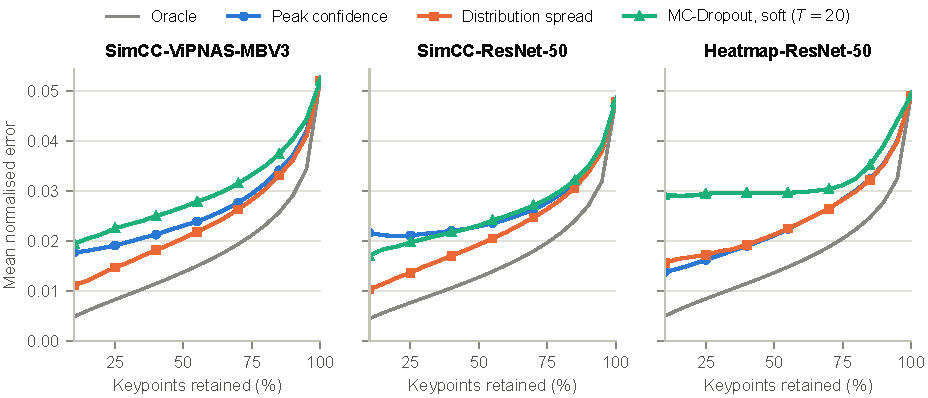
\includegraphics[width=\linewidth]{sparsification.pdf}
\caption{Sparsification on the test split: mean error of the keypoints retained after discarding
the most uncertain ones. Lower is better, and the oracle sorts by the true error. Values are in
Table~\ref{tab:zeroshot} (AUSE).}
\label{fig:sparsification}
\end{figure}

\paragraph{Dropout rate} The planned rate of $0.1$ could have been a poor choice, so we repeated
inference at $p\in\{0.05,0.2,0.3,0.5\}$ (exploratory). The best MC-Dropout result over all rates and
both decoders was \SweepBestZsSimccMbvThree{} on ViPNAS-MobileNetV3 (\SweepBestVariantZsSimccMbvThree{},
$p{=}\SweepBestRateZsSimccMbvThree$), \SweepBestZsSimccRFiveZero{} on ResNet-50
(\SweepBestVariantZsSimccRFiveZero{}, $p{=}\SweepBestRateZsSimccRFiveZero$), and
\SweepBestZsHmRFiveZero{} on the heatmap model (\SweepBestVariantZsHmRFiveZero{},
$p{=}\SweepBestRateZsHmRFiveZero$). All are below the corresponding best one-pass signal
(Table~\ref{tab:sweep}, Figure~\ref{fig:sweep}). No rate closes the gap.

\begin{table}[t]
\centering\small
\caption{Failure AUROC of soft MC-Dropout ($T{=}20$) by dropout rate, against one-pass spread.
Exploratory. Figure~\ref{fig:sweep} also shows the argmax decoder.}
\label{tab:sweep}
\adjustbox{max width=\linewidth}{\begin{tabular}{lcccccc}
\toprule
Model & $p{=}0.05$ & $p{=}0.1$ & $p{=}0.2$ & $p{=}0.3$ & $p{=}0.5$ & Spread (1 pass) \\
\midrule
SimCC-ViPNAS-MBV3 & 0.817 & 0.820 & 0.822 & 0.823 & 0.822 & 0.913 \\
SimCC-ResNet-50 & 0.873 & 0.873 & 0.874 & 0.873 & 0.871 & 0.914 \\
Heatmap-ResNet-50 & 0.819 & 0.827 & 0.812 & 0.782 & 0.699 & 0.905 \\
\bottomrule
\end{tabular}
}
\end{table}

\begin{figure}[t]
\centering
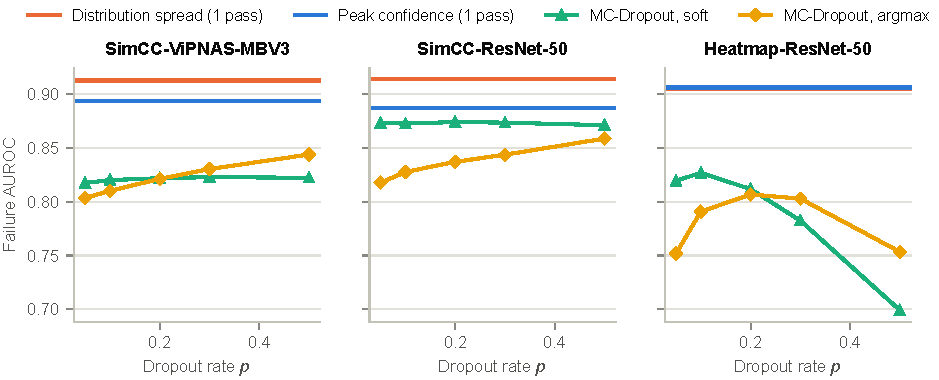
\includegraphics[width=\linewidth]{sweep.pdf}
\caption{Failure AUROC against dropout rate. One-pass signals are flat lines because they do not
depend on the rate.}
\label{fig:sweep}
\end{figure}

\paragraph{Flip testing} Table~\ref{tab:zeroshot} uses flip-test predictions, so its one-pass
signals in fact come from two backbone passes. With flip testing off (exploratory), spread reached
\FaNoflipZsSimccMbvThreeDist{} and \FaNoflipZsSimccRFiveZeroDist{} on SimCC, and peak confidence
\FaNoflipZsHmRFiveZeroConf{} on the heatmap model, against \FaNoflipZsSimccMbvThreeMcSoft{},
\FaNoflipZsSimccRFiveZeroMcSoft{} and \FaNoflipZsHmRFiveZeroMcSoft{} for soft MC-Dropout, so the
one-pass claim holds in the strict sense too.

\paragraph{Occlusion} Occlusion AUROC follows the same pattern, at a lower level. The best
signal reached \OaZsSimccMbvThreeFusion{}, \OaZsSimccRFiveZeroFusion{} and \OaZsHmRFiveZeroDist{}
on the three models, compared with \OaZsSimccMbvThreeMcSoft{}, \OaZsSimccRFiveZeroMcSoft{} and
\OaZsHmRFiveZeroMcSoft{} for soft MC-Dropout. Figure~\ref{fig:qualitative} shows instances selected
by a fixed rule, not by hand.

\begin{figure}[t]
\centering
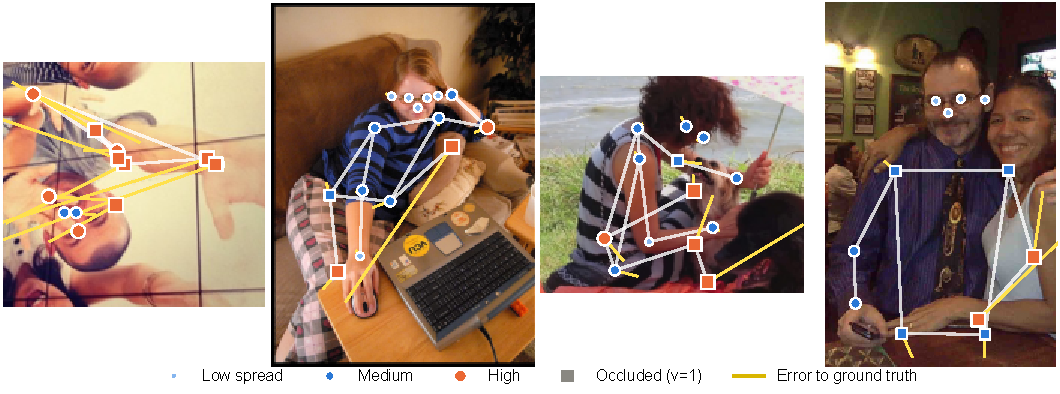
\includegraphics[width=\linewidth]{qualitative.pdf}
\caption{SimCC ViPNAS-MobileNetV3 on test instances chosen by rule: of those with at least 3
occluded and 6 visible labelled joints and a box side of at least 150 pixels, the four with the
largest gap between occluded and visible mean error. These are selected failures and do not show
typical accuracy.}
\label{fig:qualitative}
\end{figure}

\subsection{Conformal error bounds}

Table~\ref{tab:conformal} gives the conformal results, with the same procedure applied to each scale.
All variants reach close to the 90\% marginal target, as the construction guarantees. A constant radius covered only
\CovOccZsSimccMbvThreeConstant{} and \CovOccZsSimccRFiveZeroConstant{} of occluded joints on SimCC.
Scaling by spread raised this to \CovOccZsSimccMbvThreeDist{} and \CovOccZsSimccRFiveZeroDist{}, and
changed the mean radius by \RadiusChangeZsSimccMbvThree\% and \RadiusChangeZsSimccRFiveZero\%. On
the heatmap model it raised occluded coverage to \CovOccZsHmRFiveZeroDist{}, but at the price of a
\RadiusChangeZsHmRFiveZero\% larger radius, so the benefit there is a trade-off and not a clear gain.
Occluded coverage remains below the marginal target in every case: this marginal guarantee does not
extend to the occluded subgroup.

\begin{table}[t]
\centering\small
\caption{Split-conformal regions at 90\% target coverage. Radii are in normalised error units.}
\label{tab:conformal}
\adjustbox{max width=\linewidth}{\begin{tabular}{llcccc}
\toprule
Model & Radius scaled by & Coverage & Vis.\ cov. & Occl.\ cov. & Mean radius \\
\midrule
SimCC-ViPNAS-MBV3 & Constant & 0.896 & 0.929 & 0.657 & 0.098 \\
 & Distribution spread & 0.901 & 0.919 & 0.770 & 0.085 \\
 & MC-Dropout, soft ($T{=}20$) & 0.900 & 0.924 & 0.719 & 0.091 \\
\addlinespace
SimCC-ResNet-50 & Constant & 0.898 & 0.931 & 0.658 & 0.091 \\
 & Distribution spread & 0.899 & 0.918 & 0.762 & 0.078 \\
 & MC-Dropout, soft ($T{=}20$) & 0.897 & 0.918 & 0.741 & 0.085 \\
\addlinespace
Heatmap-ResNet-50 & Constant & 0.896 & 0.932 & 0.641 & 0.090 \\
 & Distribution spread & 0.902 & 0.906 & 0.875 & 0.132 \\
 & MC-Dropout, soft ($T{=}20$) & 0.900 & 0.910 & 0.822 & 0.135 \\
\addlinespace
\bottomrule
\end{tabular}
}
\end{table}

\subsection{Current lightweight models: RTMPose}\label{sec:rtmpose}

RTMPose~\cite{jiang2023rtmpose} is the current family of real-time SimCC-style models. We evaluated its
published COCO checkpoints at three sizes, from RTMPose-t (\ParamsRtmposeT{}\,M parameters,
\FlopsRtmposeT{}\,GFLOPs, \CpuOneRtmposeT{}\,ms per person on one CPU thread) to RTMPose-m, with the same
split, signals and metrics as above and no retraining (Table~\ref{tab:rtmpose}). This evaluation was
added after the main study. With detector boxes our pipeline reproduced the published AP to within 0.2
points (\ApDetZsRtmposeT{}, \ApDetZsRtmposeS{} and \ApDetZsRtmposeM{} against \ApPubZsRtmposeT{},
\ApPubZsRtmposeS{} and \ApPubZsRtmposeM{}). \method{} adds \MethodCpuPctRtmT\% to the CPU time of
RTMPose-t.

Three findings carry over and one does not. \method{}'s score again beat 20-pass head MC-Dropout on
every model, by \DfaZsRtmposeTDistMinusMc{}, \DfaZsRtmposeSDistMinusMc{} and \DfaZsRtmposeMDistMinusMc{}
in failure AUROC, though the gap narrows as the model grows. It detected occluded joints better than the
default confidence on every model, by \DoaZsRtmposeTDistMinusConf{}, \DoaZsRtmposeSDistMinusConf{} and
\DoaZsRtmposeMDistMinusConf{} in occlusion AUROC. And its conformal bounds changed the mean radius by
\RtmRadiusRange\% against a constant radius while raising coverage of occluded joints, for RTMPose-t from
\CovOccZsRtmposeTConstant{} to \CovOccZsRtmposeTDist{}. What did not carry over is the gain over the
default confidence in failure detection: on RTMPose the two could not be separated
(\DfaZsRtmposeTDistMinusConf{}, \DfaZsRtmposeSDistMinusConf{} and \DfaZsRtmposeMDistMinusConf{}), and the
default confidence had the lower AUSE (spread minus confidence \DauseZsRtmposeTDistMinusConf{} on
RTMPose-t, $\times10^{-3}$). RTMPose's loss applies a softmax to its Gaussian targets and a temperature
to its logits, which may give its default score a better ranking than the original SimCC models have;
we did not test this. The spread
was also not the best single signal there: entropy was ahead on RTMPose-t
(\DfaZsRtmposeTEntropyMinusDist{}) and logistic fusion on RTMPose-t and RTMPose-s
(\DfaZsRtmposeTFusionMinusDist{} and \DfaZsRtmposeSFusionMinusDist{}), while the spread led entropy on
occlusion on all three. We keep the spread as defined before these models were seen. Rescoring did not
help on RTMPose: calibration selected little or no exponential decay ($\Delta$AP \RtmRescoreExpAlphaDistGt{}
points with ground-truth boxes), and expected OKS lowered AP by \RtmRescoreEoksDistGt{} and
\RtmRescoreEoksDistDet{} points with ground-truth and detector boxes.

\begin{table}[t]
\centering\small
\caption{RTMPose with published COCO weights, no retraining. AP is on all val2017 images as a
reproduction check; uncertainty metrics are on the test split. ``Spread minus'' columns are paired
failure AUROC differences. Occluded coverage is for 90\% conformal regions with a constant radius and
with \method{}'s spread. $^\dagger$MMPose model zoo values with a different detector, not re-measured.}
\label{tab:rtmpose}
\adjustbox{max width=\linewidth}{\begin{tabular}{lcccccccccc}
\toprule
& \multicolumn{3}{c}{AP, all val2017} & \multicolumn{3}{c}{Failure AUROC} & \multicolumn{2}{c}{Spread minus} & \multicolumn{2}{c}{Occl.\ coverage} \\
\cmidrule(lr){2-4}\cmidrule(lr){5-7}\cmidrule(lr){8-9}\cmidrule(lr){10-11}
Model & GT & det. & Publ.$^{\dagger}$ & Peak conf. & Spread & MC soft & MC soft & Peak conf. & Const. & Spread \\
\midrule
RTMPose-t & 0.697 & 0.680 & 0.682 & 0.900 & 0.902 & 0.886 & +0.017 & +0.002 & 0.653 & 0.786 \\
RTMPose-s & 0.733 & 0.714 & 0.716 & 0.906 & 0.909 & 0.896 & +0.013 & +0.003 & 0.645 & 0.793 \\
RTMPose-m & 0.766 & 0.746 & 0.746 & 0.907 & 0.910 & 0.904 & +0.006 & +0.003 & 0.656 & 0.796 \\
\bottomrule
\end{tabular}
}
\end{table}

\subsection{Cross-dataset test under heavy occlusion: OCHuman}\label{sec:ochuman}

OCHuman~\cite{zhang2019pose2seg} shows people heavily occluded by other people. We ran the six published
COCO models on it without retraining and used its official split: every fitted quantity on OCHuman val
(\ochNumCalImages{} images) and every reported value on OCHuman test (\ochNumTestImages{} images,
\ochNumKptTest{} labelled keypoints, of which \ochNumOccTest{} occluded). This evaluation was planned
and logged before any OCHuman result was computed. The models are much less accurate here: PCK@0.1 on
occluded joints was \PckOccOchSimccMbvThree{} for SimCC-ViPNAS-MobileNetV3 and \PckOccOchRtmposeM{} for
RTMPose-m, against \PckVisOchSimccMbvThree{} and \PckVisOchRtmposeM{} on visible ones. Every signal was
weaker as well: the best failure AUROC per model was \ochBestFaRange{}, against \cocoBestFaRange{} on COCO
(Table~\ref{tab:ochuman}).

Two COCO findings held. \method{}'s score beat 20-pass MC-Dropout on all \ochNumSimcc{} SimCC-style
models, from \DfaOchRtmposeM{} on RTMPose-m to \DfaOchSimccMbvThree{} on SimCC-ViPNAS-MobileNetV3, and it
again beat the default confidence on the original SimCC models (\DfaconfOchSimccMbvThree{} and
\DfaconfOchSimccRFiveZero{}) while matching it on RTMPose. The conformal bounds kept their coverage under
this harder distribution, from \ochCoverageRange{} for every model and scale, and against the
constant radius \method{} changed the mean radius by \ochRadiusRange\% on the SimCC-style models at about
the same occluded coverage (for SimCC-ViPNAS-MobileNetV3, \CovOccOchSimccMbvThreeDist{} against
\CovOccOchSimccMbvThreeConstant{}). Here the gain is a tighter bound at equal coverage, where on COCO it
was higher occluded coverage.

One finding reversed. On OCHuman the spread detected occluded joints \emph{worse} than the default
confidence on every SimCC-style model, by \DoaconfOchSimccMbvThree{} on SimCC-ViPNAS-MobileNetV3 and
\DoaconfOchRtmposeM{} on RTMPose-m, where on COCO it had been better on all five. We did not test why. One
possibility is that a joint hidden by another person often produces a sharp distribution on that
person's joint, a confident error that a dispersion score cannot see. Occlusion detection should
therefore not be read as a general property of \method{}. On the heatmap model the conformal radius grew
by \RadiusChangeOchHmRFiveZero\%, as on COCO.

\begin{table}[t]
\centering\small
\caption{OCHuman test, COCO-trained models without retraining, all fitting on OCHuman val. PCK is
PCK@0.1 on occluded joints. ``Spread minus'' columns are paired failure AUROC differences, and the
occlusion column the paired occlusion AUROC difference. Occluded coverage is for 90\% conformal regions.
$^\ast$Heatmap model, for which the spread is not \method{}'s SimCC score.}
\label{tab:ochuman}
\adjustbox{max width=\linewidth}{\begin{tabular}{lccccccccc}
\toprule
& & \multicolumn{3}{c}{Failure AUROC} & \multicolumn{2}{c}{Spread minus} & Occl.\ AUROC & \multicolumn{2}{c}{Occl.\ coverage} \\
\cmidrule(lr){3-5}\cmidrule(lr){6-7}\cmidrule(lr){9-10}
Model & PCK occl. & Peak conf. & Spread & MC soft & MC soft & Peak conf. & spread $-$ conf. & Const. & Spread \\
\midrule
SimCC-ViPNAS-MBV3 & 0.425 & 0.736 & 0.750 & 0.690 & +0.059 & +0.013 & \ensuremath{-}0.016 & 0.850 & 0.848 \\
SimCC-ResNet-50 & 0.406 & 0.734 & 0.744 & 0.716 & +0.029 & +0.011 & \ensuremath{-}0.022 & 0.842 & 0.837 \\
Heatmap-ResNet-50$^{\ast}$ & 0.422 & 0.721 & 0.721 & 0.658 & +0.062 & \ensuremath{-}0.001 & \ensuremath{-}0.005 & 0.840 & 0.844 \\
RTMPose-t & 0.419 & 0.770 & 0.771 & 0.741 & +0.030 & +0.001 & \ensuremath{-}0.044 & 0.840 & 0.850 \\
RTMPose-s & 0.439 & 0.767 & 0.765 & 0.734 & +0.031 & \ensuremath{-}0.002 & \ensuremath{-}0.057 & 0.837 & 0.843 \\
RTMPose-m & 0.457 & 0.759 & 0.761 & 0.743 & +0.019 & +0.002 & \ensuremath{-}0.058 & 0.837 & 0.841 \\
\bottomrule
\end{tabular}
}
\end{table}

\subsection{Comparison with a trained uncertainty head}\label{sec:headcmp}

Could training for uncertainty beat a score that needs no training? This section fine-tunes the
baseline head of Section~\ref{sec:learned} on the same backbones and compares its learned outputs
with \method{}'s score computed on the same fine-tuned model, so both see identical weights.

\paragraph{The control, and MC-Dropout after training} The \texttt{base} arm fine-tunes the
ViPNAS-MobileNetV3 model for 20 epochs with KL only and head dropout active. Its AP on all val2017
images was \ApGtFtMbvThreeBaseSZero{} with ground-truth boxes (pretrained: \ApGtZsSimccMbvThree{}) and
\ApDetFtMbvThreeBaseSZero{} with detector boxes (pretrained: \ApDetZsSimccMbvThree{}), so the
fine-tuning schedule itself does no harm. Training with dropout did help MC-Dropout: failure AUROC rose
from \FaZsSimccMbvThreeMcSoft{} to \FaFtMbvThreeBaseSZeroMcSoft{} for the soft decoder and from
\FaZsSimccMbvThreeMc{} to \FaFtMbvThreeBaseSZeroMc{} for argmax, and occlusion AUROC from
\OaZsSimccMbvThreeMcSoft{} to \OaFtMbvThreeBaseSZeroMcSoft{}. The pretrained comparison in
Table~\ref{tab:zeroshot} is therefore somewhat unfavourable to MC-Dropout. The ranking did not change:
spread reached \FaFtMbvThreeBaseSZeroDist{} on the same model, and soft MC-Dropout minus spread was
\DfaFtMbvThreeBaseSZeroMcSoftMinusDist{}. This is one seed on one backbone.

\paragraph{The full learned head} The \texttt{full} arm adds the heteroscedastic, calibration and OKS
terms, the token mixer and the adaptive target. Table~\ref{tab:ablation} compares it with the control.
On ViPNAS-MobileNetV3 with seed 0 (other seeds below), the learned signals did not beat spread computed
on the same model's output. Learned $\sigma$ minus spread was \DfaFtMbvThreeFullSZeroHetMinusDist{} in failure
AUROC, \DauseFtMbvThreeFullSZeroHetMinusDist{} in AUSE ($\times 10^{-3}$, lower is better) and
\DoaFtMbvThreeFullSZeroHetMinusDist{} in occlusion AUROC, so $\sigma$ was worse on the first two and
not distinguishable on the third. The OKS head was further behind, at
\DfaFtMbvThreeFullSZeroOksMinusDist{} in failure AUROC. Adding both to logistic fusion did not separate
it from spread alone either (\DfaFtMbvThreeFullSZeroFusionMinusDist{}).

The head also cost accuracy. On val-test, AP with ground-truth boxes was \ApTestGtFtMbvThreeFullSZero{}
against \ApTestGtFtMbvThreeBaseSZero{} for the control, a mean paired fold difference of
\DapGtFtMbvThreeFullSZero{} $\pm$ \DapSdGtFtMbvThreeFullSZero{} AP points, positive in
\DapPosGtFtMbvThreeFullSZero{} folds. With detector boxes the difference was
\DapDetFtMbvThreeFullSZero{} $\pm$ \DapSdDetFtMbvThreeFullSZero{} points. So the deficit seen at the
interim check did not close by the final epoch. The median logged gradient norm before clipping, where
each logged value is a 50-iteration mean, was \GradNormFtMbvThreeFullSZero{} for \texttt{full} and
\GradNormFtMbvThreeBaseSZero{} for the control, against a clip threshold of 1.0.

\begin{table}[t]
\centering\small
\caption{Fine-tuning arms, final-epoch checkpoints. AP is on val-test images. $\Delta$ is the mean
paired difference from the control across 10 disjoint val-test folds, in AP points, with the SD across
folds, for ground-truth (GT) and detector (det.) boxes. $^{\S}$Exploratory arm, added after an interim
look at evaluation data (Section~\ref{sec:arms}).}
\label{tab:ablation}
\adjustbox{max width=\linewidth}{\begin{tabular}{llcccccccc}
\toprule
& & \multicolumn{3}{c}{AP, val-test} & \multicolumn{3}{c}{Failure AUROC} & \multicolumn{2}{c}{Occlusion AUROC} \\
\cmidrule(lr){3-5}\cmidrule(lr){6-8}\cmidrule(lr){9-10}
Backbone & Arm & GT & $\Delta$ GT & $\Delta$ det. & Spread & Learned $\sigma$ & Learned OKS & Spread & Learned $\sigma$ \\
\midrule
ViPNAS-MBV3 & Pretrained & 0.717 & \ensuremath{-}0.24 $\pm$ 0.22 & \ensuremath{-}0.18 $\pm$ 0.14 & 0.913 & -- & -- & 0.798 & -- \\
 & Control (KL only) & 0.720 & -- & -- & 0.912 & -- & -- & 0.799 & -- \\
 & + $\sigma$ head & 0.709 & \ensuremath{-}1.09 $\pm$ 0.60 & \ensuremath{-}0.84 $\pm$ 0.59 & 0.912 & 0.907 & -- & 0.799 & 0.800 \\
 & + OKS head & 0.710 & \ensuremath{-}0.94 $\pm$ 0.47 & \ensuremath{-}0.86 $\pm$ 0.43 & 0.912 & 0.907 & 0.868 & 0.798 & 0.799 \\
 & + Token mixer & 0.713 & \ensuremath{-}0.75 $\pm$ 0.48 & \ensuremath{-}0.54 $\pm$ 0.29 & 0.909 & 0.903 & 0.868 & 0.799 & 0.800 \\
 & + Adaptive target & 0.708 & \ensuremath{-}1.24 $\pm$ 0.56 & \ensuremath{-}1.03 $\pm$ 0.40 & 0.913 & 0.904 & 0.868 & 0.796 & 0.798 \\
 & Same, stop-gradient$^{\S}$ & 0.715 & \ensuremath{-}0.38 $\pm$ 0.34 & \ensuremath{-}0.40 $\pm$ 0.27 & 0.909 & 0.905 & 0.868 & 0.796 & 0.799 \\
\midrule
ResNet-50 & Pretrained & 0.741 & +0.04 $\pm$ 0.19 & \ensuremath{-}0.07 $\pm$ 0.21 & 0.914 & -- & -- & 0.801 & -- \\
 & Control (KL only) & 0.741 & -- & -- & 0.915 & -- & -- & 0.801 & -- \\
 & + Adaptive target & 0.740 & \ensuremath{-}0.26 $\pm$ 0.31 & \ensuremath{-}0.15 $\pm$ 0.39 & 0.914 & 0.898 & 0.857 & 0.801 & 0.796 \\
\bottomrule
\end{tabular}
}
\end{table}

\paragraph{Stopping the pose gradient (exploratory)} The \texttt{full\_sg} arm detaches $D$ in
$\mathcal{L}_{\text{het}}$ and is otherwise identical to \texttt{full}. Its logged gradient norm stayed
large, with a median of \GradNormFtMbvThreeFullSgSZero{}, so the detach did not remove the large norms that
prompted this arm. On val-test its AP was \ApTestGtFtMbvThreeFullSgSZero{} with
ground-truth boxes, \DapGtFtMbvThreeFullSgSZero{} $\pm$ \DapSdGtFtMbvThreeFullSgSZero{} points from the
control and \DapSgVsFullGt{} $\pm$ \DapSdSgVsFullGt{} from \texttt{full} (positive in
\DapPosSgVsFullGt{} folds). With detector boxes these were \DapDetFtMbvThreeFullSgSZero{} $\pm$
\DapSdDetFtMbvThreeFullSgSZero{} and \DapSgVsFullDet{} $\pm$ \DapSdSgVsFullDet{} (positive in
\DapPosSgVsFullDet{} folds). So on this seed the detach removed most of the AP loss, though not all of
it. It did not change the ranking of the signals. Learned $\sigma$ minus spread was
\DfaFtMbvThreeFullSgSZeroHetMinusDist{} in failure AUROC and \DauseFtMbvThreeFullSgSZeroHetMinusDist{} in
AUSE, and only on occlusion AUROC did $\sigma$ come out ahead, by \DoaFtMbvThreeFullSgSZeroHetMinusDist{}.
That occlusion difference is small. An evaluation-set number prompted this arm and it has one seed, so the
AP recovery is a hypothesis for later work and not an established result.

\paragraph{ResNet-50} The larger backbone repeats the signal result but not the size of the AP cost, on
one seed. Learned $\sigma$ minus spread was \DfaFtRFiveZeroFullSZeroHetMinusDist{} in failure AUROC,
\DauseFtRFiveZeroFullSZeroHetMinusDist{} in AUSE and \DoaFtRFiveZeroFullSZeroHetMinusDist{} in occlusion
AUROC, so here $\sigma$ was worse on all three. The OKS head was at
\DfaFtRFiveZeroFullSZeroOksMinusDist{} in failure AUROC, and fusion with both learned signals was not
separated from spread (\DfaFtRFiveZeroFullSZeroFusionMinusDist{}). The AP difference from the control was
\DapGtFtRFiveZeroFullSZero{} $\pm$ \DapSdGtFtRFiveZeroFullSZero{} points with ground-truth boxes and
\DapDetFtRFiveZeroFullSZero{} $\pm$ \DapSdDetFtRFiveZeroFullSZero{} with detector boxes, each smaller than
its SD across folds, so we cannot call it a cost on this backbone. Training with dropout again helped
MC-Dropout, from \FaZsSimccRFiveZeroMcSoft{} to \FaFtRFiveZeroBaseSZeroMcSoft{} for the soft decoder, but
it stayed behind spread (\DfaFtRFiveZeroBaseSZeroMcSoftMinusDist{}).

\paragraph{Which component costs AP} The planned arms on ViPNAS-MobileNetV3 add one component at a time,
on one seed. The first step carried most of the loss: \texttt{het}, which adds only the $\sigma$ head with
$\mathcal{L}_{\text{het}}$ and $\mathcal{L}_{\text{cal}}$, differed from the control by
\DapGtFtMbvThreeHetSZero{} $\pm$ \DapSdGtFtMbvThreeHetSZero{} points with ground-truth boxes (positive in
\DapPosGtFtMbvThreeHetSZero{} folds) and \DapDetFtMbvThreeHetSZero{} $\pm$ \DapSdDetFtMbvThreeHetSZero{}
with detector boxes. Measured directly against the arm before each, with ground-truth boxes, the OKS head
changed AP by \StepGtFtMbvThreeHetOksSZero{} $\pm$ \StepSdGtFtMbvThreeHetOksSZero{} (positive in
\StepPosGtFtMbvThreeHetOksSZero{} folds), the token mixer by \StepGtFtMbvThreeMixSZero{} $\pm$
\StepSdGtFtMbvThreeMixSZero{} (\StepPosGtFtMbvThreeMixSZero{}) and the adaptive target by
\StepGtFtMbvThreeFullSZero{} $\pm$ \StepSdGtFtMbvThreeFullSZero{} (\StepPosGtFtMbvThreeFullSZero{}). With
detector boxes the adaptive-target step was \StepDetFtMbvThreeFullSZero{} $\pm$
\StepSdDetFtMbvThreeFullSZero{} (\StepPosDetFtMbvThreeFullSZero{}). So the heteroscedastic and calibration
terms are the main source of the cost, the OKS head shows no effect, and the adaptive target may add to it.
These later steps are about the size of their fold SD, and folds capture image sampling but not variation
between training runs, so they are weak evidence on one seed.

No arm brought learned $\sigma$ level with spread on failure AUROC. The difference was
\DfaFtMbvThreeHetSZeroHetMinusDist{} for \texttt{het}, \DfaFtMbvThreeHetOksSZeroHetMinusDist{} for
\texttt{het\_oks} and \DfaFtMbvThreeMixSZeroHetMinusDist{} for \texttt{mix}. On occlusion AUROC these three
arms could not be separated from spread (\DoaFtMbvThreeHetSZeroHetMinusDist{},
\DoaFtMbvThreeHetOksSZeroHetMinusDist{} and \DoaFtMbvThreeMixSZeroHetMinusDist{}). The added components did
not improve the signal either: $\sigma$ scored \FaFtMbvThreeHetSZeroHet{} in the simplest arm and
\FaFtMbvThreeFullSZeroHet{} in \texttt{full}.

\begin{figure}[t]
\centering
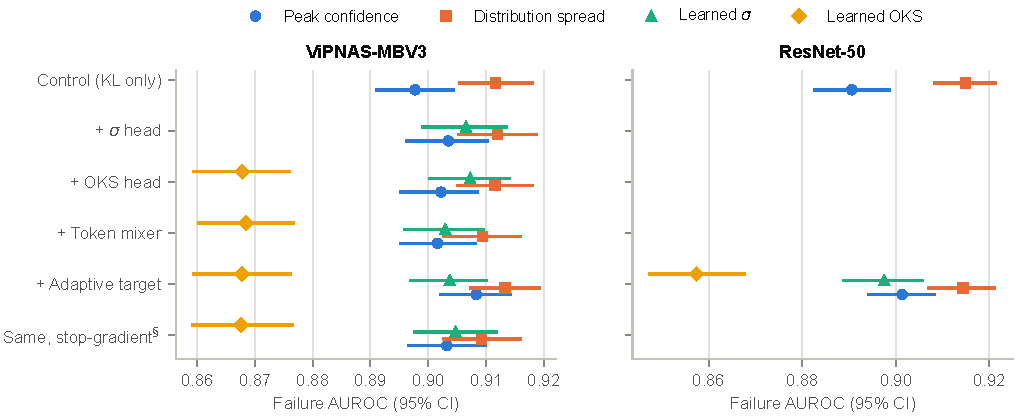
\includegraphics[width=\linewidth]{ablation.pdf}
\caption{Failure AUROC on val-test for each fine-tuning arm, one seed, with 95\% bootstrap intervals.
Intervals from different signals on the same images are not independent, so paired differences in the
text are the proper comparison. $^{\S}$Exploratory arm.}
\label{fig:ablation}
\end{figure}

\paragraph{Repeated training runs} We trained \texttt{base} and \texttt{full} on ViPNAS-MobileNetV3 again
with seeds 1 and 2 (Table~\ref{tab:seeds}). Each seed's AP difference is the paired fold mean against the
control trained with the same seed, so the spread across seeds reflects variation between training runs,
which the fold SD does not capture. The AP cost appeared on every seed: \SeedDapGt{} $\pm$ \SeedDapSdGt{}
points with ground-truth boxes (mean and SD over \SeedCount{} seeds, range \SeedDapRangeGt{}) and
\SeedDapDet{} $\pm$ \SeedDapSdDet{} with detector boxes (range \SeedDapRangeDet{}). The control itself was
stable, at \ApTestGtFtMbvThreeBaseSZero{}, \ApTestGtFtMbvThreeBaseSOne{} and \ApTestGtFtMbvThreeBaseSTwo{}.
The signal ranking also held. Learned $\sigma$ minus spread in failure AUROC was \SeedDfaHetMinusDist{}
$\pm$ \SeedDfaHetMinusDistSd{} across seeds, with the 95\% interval below zero in
\SeedDfaHetMinusDistBelow{} seeds. For the OKS head it was \SeedDfaOksMinusDist{} $\pm$
\SeedDfaOksMinusDistSd{}, below zero in \SeedDfaOksMinusDistBelow{}. On occlusion AUROC, $\sigma$ minus
spread averaged \SeedDoaHetMinusDist{}, with the interval above zero in \SeedDoaHetMinusDistAbove{} seeds
and below zero in \SeedDoaHetMinusDistBelow{}. Three seeds give a rough estimate of run-to-run variation,
not a precise one, and the ablation arms, \texttt{full\_sg} and ResNet-50 remain single runs.

\begin{table}[t]
\centering\small
\caption{Seeds 0, 1 and 2 of the control and the full head on ViPNAS-MobileNetV3, mean $\pm$ SD across
seeds. AP is on val-test with ground-truth boxes. $\Delta$ is each seed's mean paired fold difference
from the control of the same seed, in AP points, then averaged across seeds. $\sigma$ and OKS are the
learned head's outputs. AUROC values are on val-test.}
\label{tab:seeds}
\adjustbox{max width=\linewidth}{\begin{tabular}{lccccccc}
\toprule
& & \multicolumn{2}{c}{AP, val-test, GT} & \multicolumn{3}{c}{Failure AUROC} & Occl.\ AUROC \\
\cmidrule(lr){3-4}\cmidrule(lr){5-7}\cmidrule(lr){8-8}
Arm & Seeds & AP & $\Delta$ & Spread & $\sigma$ & OKS & Spread \\
\midrule
Control (KL only) & 3 & 0.7198 $\pm$ 0.0004 & -- & 0.911 $\pm$ 0.000 & -- & -- & 0.798 $\pm$ 0.000 \\
Full head & 3 & 0.7096 $\pm$ 0.0017 & \ensuremath{-}1.07 $\pm$ 0.16 & 0.911 $\pm$ 0.002 & 0.903 $\pm$ 0.001 & 0.868 $\pm$ 0.001 & 0.797 $\pm$ 0.000 \\
\bottomrule
\end{tabular}
}
\end{table}

\subsection{Cost}\label{sec:cost}

\method{} adds a median of \MethodCpuMs{}\,ms per person on one CPU thread and at most
\MethodGpuMs{}\,ms on the GPU, which is \MethodCpuPct\% and \MethodGpuPct\% of a single forward pass of
the plain ViPNAS-MobileNetV3 model (\CpuOneMbvThreePlain{}\,ms and \GpuOneMbvThreePlain{}\,ms). It adds
no parameters and no FLOPs that matter at this scale, and no training.

Table~\ref{tab:cost} gives the cost of the baselines. The trained head adds little in FLOPs: from
\FlopsMbvThreePlain{}\,G to \FlopsMbvThreeFull{}\,G on ViPNAS-MobileNetV3 including the mixer. Its
parameter overhead matters more on the lightweight model, from \ParamsMbvThreePlain{}\,M to
\ParamsMbvThreeFull{}\,M. Head-only MC-Dropout with $T{=}20$ costs far less than 20 forward passes
because the backbone runs once: \GpuRatioMbvThreeHetOks{}$\times$ to \GpuRatioHmRFiveZero{}$\times$ a single
pass on the GPU, and \CpuRatioMbvThreeHetOks{}$\times$ to \CpuRatioHmRFiveZero{}$\times$ on one CPU thread.
So the case for \method{} over head MC-Dropout rests mainly on its stronger signal and not on latency,
and any argument based on an assumed $20\times$ cost overstates the difference. The AP cost of the
trained head is reported in Section~\ref{sec:headcmp}.

\begin{table}[t]
\centering\scriptsize
\caption{Model cost at batch size 1, median over 300 runs. ``Ratio'' is $T{=}20$ time over single-pass
time on the GPU. $^\ddagger$Includes the unused uncertainty modules of our head.
Sub-10\,ms GPU differences should be read with caution, since desktop applications shared the GPU.}
\label{tab:cost}
\adjustbox{max width=\linewidth}{\begin{tabular}{lrrrrrrr}
\toprule
& Params & FLOPs & \multicolumn{2}{c}{GPU (ms)} & & \multicolumn{2}{c}{CPU, 1 thread (ms)} \\
Model & (M) & (G) & 1 pass & $T{=}20$ & Ratio & 1 pass & $T{=}20$ \\
\midrule
ViPNAS-MBV3, plain SimCC & 8.65 & 0.80 & 10.7 & -- & -- & 49 & -- \\
ViPNAS-MBV3, + $\sigma$/OKS head & 9.06 & 0.80 & 10.2 & 27.8 & 2.7$\times$ & 50 & 107 \\
ViPNAS-MBV3, + token mixer & 9.62 & 0.82 & 12.6 & 41.8 & 3.3$\times$ & 50 & 128 \\
ResNet-50, plain SimCC & 36.75 & 5.50 & 4.9 & -- & -- & 123 & -- \\
ResNet-50, + $\sigma$/OKS head & 37.16 & 5.50 & 5.5 & 21.9 & 4.0$\times$ & 122 & 854 \\
ResNet-50, + token mixer & 37.72 & 5.51 & 8.1 & 39.8 & 4.9$\times$ & 123 & 906 \\
ResNet-34, SimCC$^{\ddagger}$ & 28.65 & 4.77 & 5.0 & 20.6 & 4.1$\times$ & 98 & 607 \\
SOCA-PRNet-34, SimCC$^{\ddagger}$ & 28.95 & 4.77 & 6.9 & 23.9 & 3.5$\times$ & 101 & 606 \\
ResNet-50, heatmap$^{\ddagger}$ & 34.30 & 5.45 & 5.4 & 28.0 & 5.2$\times$ & 138 & 1235 \\
RTMPose-t & 3.34 & 0.36 & 4.6 & 25.8 & 5.6$\times$ & 14 & 38 \\
RTMPose-s & 5.47 & 0.68 & 4.9 & 25.6 & 5.3$\times$ & 21 & 46 \\
RTMPose-m & 13.59 & 1.93 & 6.7 & 30.6 & 4.5$\times$ & 46 & 78 \\
\bottomrule
\end{tabular}
}
\end{table}

\subsection{Instance rescoring}

Can the same score also raise COCO AP? Table~\ref{tab:rescoring} shows small AP changes. Exponential decay on spread gained
\DapZsSimccMbvThreeExpAlphaDist{} and \DapZsSimccRFiveZeroExpAlphaDist{} AP points with ground-truth
boxes, and \DapZsSimccMbvThreeDetExpAlphaDist{} and \DapZsSimccRFiveZeroDetExpAlphaDist{} with detector
boxes, with fold standard deviations of similar size. Expected OKS changed AP by
\DapZsSimccMbvThreeEoksDist{} and \DapZsSimccRFiveZeroEoksDist{} points with ground-truth boxes, and
by \DapZsSimccMbvThreeDetEoksDist{} and \DapZsSimccRFiveZeroDetEoksDist{} with detector boxes. On the
heatmap model, calibration selected $\alpha=\SelAlphaZsHmRFiveZero$ for both box types, meaning no
rescoring. Spread-based rescoring is therefore not a
meaningful source of AP on these models. Its value lies in identifying which keypoints to distrust.

The fine-tuned \texttt{full} heads add two rules that use the learned outputs, expected OKS from
$\sigma$ and the predicted OKS itself, with parameters again selected on val-cal. On ViPNAS-MobileNetV3
neither helped: expected OKS from $\sigma$ changed AP by \DapFtMbvThreeFullSZeroEoksHet{} and
\DapFtMbvThreeFullSZeroDetEoksHet{} points with ground-truth and detector boxes, and the predicted OKS by
\DapFtMbvThreeFullSZeroPredOks{} $\pm$ \DapSdFtMbvThreeFullSZeroPredOks{} and
\DapFtMbvThreeFullSZeroDetPredOks{} $\pm$ \DapSdFtMbvThreeFullSZeroDetPredOks{} (positive in
\DapPosFtMbvThreeFullSZeroDetPredOks{} folds). On ResNet-50, expected OKS from $\sigma$ gained
\DapFtRFiveZeroFullSZeroEoksHet{} $\pm$ \DapSdFtRFiveZeroFullSZeroEoksHet{} points with ground-truth boxes
and \DapFtRFiveZeroFullSZeroDetEoksHet{} $\pm$ \DapSdFtRFiveZeroFullSZeroDetEoksHet{} with detector boxes
(positive in \DapPosFtRFiveZeroFullSZeroDetEoksHet{} folds), the only rescoring gain in this study that
clearly exceeds its fold SD. It comes from one training run, among several rules and models, so we treat
it as a lead to test with more seeds and not as an established gain. It is also smaller than the AP that
the head cost on the lightweight backbone.

\begin{table}[t]
\centering\scriptsize
\caption{Instance rescoring on the test split, with parameters selected on the calibration split, for
the pretrained SimCC models and the fine-tuned full heads (seed 0). All models use SimCC.
$\Delta$AP is in percentage points, paired over 10 folds. Test AP differs from
Table~\ref{tab:sanity} because it covers the test images only.}
\label{tab:rescoring}
\adjustbox{max width=\linewidth}{\begin{tabular}{llcccc}
\toprule
Model & Boxes & Rule & Test AP & $\Delta$AP (mean $\pm$ SD, 10 folds) & Folds $>0$ \\
\midrule
ViPNAS-MBV3, pretrained & GT & Default & 0.717 & -- & -- \\
 &  & Exp.\ decay (spread) & 0.719 & +0.16 $\pm$ 0.17 & 9/10 \\
 &  & E[OKS] (spread) & 0.719 & +0.14 $\pm$ 0.09 & 9/10 \\
\addlinespace
 & Det. & Default & 0.698 & -- & -- \\
 &  & Exp.\ decay (spread) & 0.700 & +0.14 $\pm$ 0.20 & 9/10 \\
 &  & E[OKS] (spread) & 0.697 & \ensuremath{-}0.08 $\pm$ 0.37 & 5/10 \\
\addlinespace
ResNet-50, pretrained & GT & Default & 0.741 & -- & -- \\
 &  & Exp.\ decay (spread) & 0.744 & +0.26 $\pm$ 0.26 & 9/10 \\
 &  & E[OKS] (spread) & 0.743 & +0.22 $\pm$ 0.15 & 10/10 \\
\addlinespace
 & Det. & Default & 0.724 & -- & -- \\
 &  & Exp.\ decay (spread) & 0.726 & +0.22 $\pm$ 0.30 & 8/10 \\
 &  & E[OKS] (spread) & 0.724 & \ensuremath{-}0.01 $\pm$ 0.30 & 4/10 \\
\addlinespace
ViPNAS-MBV3, full head & GT & Default & 0.708 & -- & -- \\
 &  & Exp.\ decay (spread) & 0.709 & +0.08 $\pm$ 0.16 & 9/10 \\
 &  & E[OKS] (spread) & 0.707 & \ensuremath{-}0.08 $\pm$ 0.09 & 3/10 \\
 &  & E[OKS] (learned $\sigma$) & 0.707 & \ensuremath{-}0.06 $\pm$ 0.12 & 4/10 \\
 &  & Learned OKS & 0.705 & \ensuremath{-}0.28 $\pm$ 0.16 & 0/10 \\
\addlinespace
 & Det. & Default & 0.690 & -- & -- \\
 &  & Exp.\ decay (spread) & 0.691 & +0.09 $\pm$ 0.20 & 8/10 \\
 &  & E[OKS] (spread) & 0.686 & \ensuremath{-}0.37 $\pm$ 0.37 & 1/10 \\
 &  & E[OKS] (learned $\sigma$) & 0.689 & \ensuremath{-}0.09 $\pm$ 0.32 & 5/10 \\
 &  & Learned OKS & 0.687 & \ensuremath{-}0.30 $\pm$ 0.26 & 0/10 \\
\addlinespace
ResNet-50, full head & GT & Default & 0.740 & -- & -- \\
 &  & Exp.\ decay (spread) & 0.742 & +0.26 $\pm$ 0.12 & 10/10 \\
 &  & E[OKS] (spread) & 0.741 & +0.12 $\pm$ 0.09 & 10/10 \\
 &  & E[OKS] (learned $\sigma$) & 0.743 & +0.27 $\pm$ 0.12 & 10/10 \\
 &  & Learned OKS & 0.741 & +0.14 $\pm$ 0.10 & 10/10 \\
\addlinespace
 & Det. & Default & 0.723 & -- & -- \\
 &  & Exp.\ decay (spread) & 0.725 & +0.14 $\pm$ 0.13 & 9/10 \\
 &  & E[OKS] (spread) & 0.721 & \ensuremath{-}0.24 $\pm$ 0.30 & 1/10 \\
 &  & E[OKS] (learned $\sigma$) & 0.728 & +0.45 $\pm$ 0.11 & 10/10 \\
 &  & Learned OKS & 0.726 & +0.23 $\pm$ 0.14 & 9/10 \\
\addlinespace
\bottomrule
\end{tabular}
}
\end{table}

\subsection{Models trained from ImageNet weights}

The published checkpoints were all trained by others. To check that \method{} does not depend on
them, we trained two SimCC models ourselves from ImageNet weights with the 60-epoch schedule of
Section~\ref{sec:arms}. The spread score again led: failure AUROC \FaImRThreeFourBaseSZeroDist{} on
ResNet-34 and \FaImSocaBaseSZeroDist{} on SOCA-PRNet-34, against \FaImRThreeFourBaseSZeroConf{} and
\FaImSocaBaseSZeroConf{} for the default peak confidence (Table~\ref{tab:soca}).

The pair also gives a side result on the backbone itself, since SOCA-PRNet-34 is ResNet-34 with
attention added. SOCA-PRNet-34 has \ParamsSocaBase{}\,M parameters against
\ParamsRThreeFourBase{}\,M, with FLOPs unchanged at two decimals (\FlopsSocaBase{}\,G and \FlopsRThreeFourBase{}\,G). On
val-test, AP with ground-truth boxes was \ApTestGtImSocaBaseSZero{} against \ApTestGtImRThreeFourBaseSZero{},
a mean paired fold difference of \DapGtImSocaBaseSZero{} $\pm$ \DapSdGtImSocaBaseSZero{} points (positive in
\DapPosGtImSocaBaseSZero{} folds). With detector boxes it was \DapDetImSocaBaseSZero{} $\pm$
\DapSdDetImSocaBaseSZero{} (positive in \DapPosDetImSocaBaseSZero{} folds). The difference leans towards
SOCA-PRNet, but each mean is smaller than its SD across folds, and with one training run per backbone the
variation between runs is not measured. Our fine-tuning seeds give only a rough guide to that variation,
since training from ImageNet weights for 60 epochs is a different setting. We therefore read this as a
small possible gain, not an established one.

\begin{table}[t]
\centering\small
\caption{ResNet-34 and SOCA-PRNet-34 with the same SimCC head, trained from ImageNet weights for 60
epochs, one run each. AP is on val-test images. The shortened schedule means these values cannot be
compared with published 210-epoch results.}
\label{tab:soca}
\adjustbox{max width=\linewidth}{\begin{tabular}{lcccccc}
\toprule
& & & \multicolumn{2}{c}{AP, val-test} & \multicolumn{2}{c}{Failure AUROC} \\
\cmidrule(lr){4-5}\cmidrule(lr){6-7}
Backbone & Params (M) & FLOPs (G) & GT & det. & Spread & Peak conf. \\
\midrule
ResNet-34 & 28.65 & 4.77 & 0.712 & 0.693 & 0.910 & 0.892 \\
SOCA-PRNet-34 & 28.95 & 4.77 & 0.715 & 0.698 & 0.913 & 0.897 \\
\bottomrule
\end{tabular}
}
\end{table}

\section{Discussion}

\paragraph{Why the spread score beats head MC-Dropout} We offer explanations, but did not test them
causally. The spread summarises ambiguity that the trained classifier has already learned to express:
an occluded joint tends to produce a wide or multi-modal distribution. Head-only dropout, by contrast,
perturbs a few layers around one fixed backbone feature, and a pretrained model was not fit under this
perturbation. Training with the dropout active narrowed the gap but did not close it
(Section~\ref{sec:headcmp}), which supports the training part of this account only partly. The remainder may reflect
that head dropout around one fixed backbone feature does not reach the sources of error that matter,
a possibility we did not test.

\paragraph{Why the learned head did not help} Again we did not test the explanation. A SimCC head is
already trained to put probability where the keypoint is, so its spread already carries much of what a
separate $\sigma$ head is asked to learn, and $\sigma$ is fit to the same training errors. The learned
outputs would then mostly restate the spread, which matches how close $\sigma$ came to it on every arm.
The AP cost points to an interaction with the pose objective: the arm that added only
$\mathcal{L}_{\text{het}}$ and $\mathcal{L}_{\text{cal}}$ carried most of the cost, and detaching the pose
term inside $\mathcal{L}_{\text{het}}$ recovered most of it, though in a single exploratory run. The
logged gradient norms stayed large with the detach, so the mechanism is not settled by our data.

\paragraph{Using \method{} in practice} A deployed SimCC model already computes the logits \method{}
needs, so adding it means a few lines of post-processing and one calibration pass over labelled images
from the target setting (we used \numCalImages{}). The failure probability can flag keypoints for a downstream
rule to ignore or for a human to check, and the conformal radius gives a tolerance in pixels that a
safety argument can use. Two cautions apply. The coverage guarantee is marginal and holds only when
deployment data resemble the calibration data, so the calibration set should come from the setting of
use, and occluded joints were covered below the target in every case. On heatmap models the default
score already performs comparably, so \method{} offers little there. These findings concern the models
and metrics tested, and do not rule out that other methods, such as deep ensembles, would do better at
a higher cost.

\paragraph{Limitations} The keypoint-level results use two datasets, COCO and OCHuman, top-down models
and ground-truth boxes, so detector errors are not reflected in them. On OCHuman the conformal bounds
were calibrated on OCHuman's own val split; we did not test calibrating on one dataset and deploying
on another, where the exchangeability behind the guarantee would not hold. MC-Dropout is limited to the head.
We did not evaluate full-network dropout or ensembles, and the backbones were not trained with
dropout. Only the control and the full head on ViPNAS-MobileNetV3 were trained with three seeds. Every
other arm, ResNet-50 and the SOCA comparison are single runs, and all training schedules are short.
COCO occlusion flags are annotator judgements. The test split is drawn from val2017, which
is a public benchmark and may have influenced the published models. Figures quoted at the third decimal
come from one split, though bootstrap intervals capture image sampling within it. Our detector differs
from the one behind the published numbers.

\section{Conclusion}

\method{} gives a SimCC pose estimator calibrated keypoint failure probabilities and conformal error
bounds without training, without added parameters and at a fraction of a millisecond per person. On
five published SimCC-style models, including RTMPose, and on both COCO and the heavily occluded OCHuman
dataset, it detected keypoint failures better than 20-pass head MC-Dropout, and its bounds kept their
coverage while being tighter than a constant radius. It beat the default confidence at failure
detection on the original SimCC models and matched it on RTMPose. It flagged occluded joints better than
the default confidence on COCO but worse on OCHuman, where occlusion by other people may cause confident
errors that no dispersion score can reveal. It held on models we trained ourselves. A trained uncertainty head, the costlier alternative, did not beat it: the learned
$\sigma$ and OKS outputs ranked failures worse than \method{}'s score on the same fine-tuned model, on two
backbones and, for the lightweight one, on three seeds, and the head cost about one AP point there.
Instance rescoring with the score did not move AP meaningfully, and on a heatmap model \method{} offered
little over the default score. For SimCC models we would therefore add \method{} first, and train an
uncertainty head only where a measured gain justifies its parameters and its AP cost.

\appendix
\section{Defects found and fixed}\label{app:defects}

We report these because each would have changed the results while the code still ran. Regression
tests for them are in \texttt{tests/test\_core.py}.
\begin{itemize}
\item \textbf{Pretrained heatmap weights failed to load}: inserting dropout as its own layer shifted
the deconvolution indices, so those weights were silently left random.
\item \textbf{Resuming started from random weights}: \texttt{--resume auto} cleared the
pretrained-checkpoint path even when no checkpoint existed to resume from.
\item \textbf{The anatomical prior in the mixer was overwritten} by the framework's weight
initialisation.
\item \textbf{ECE was computed on raw logits}, not on probabilities, and on the same data used for
fitting.
\item \textbf{Ties in AUROC and risk-coverage} were ordered arbitrarily, which matters because argmax
MC-Dropout often ties at zero.
\item \textbf{Inconsistent units}: the residual used for calibration and the OKS target were not on
the scale their formulas assumed. Unlabelled joints also received an OKS target.
\end{itemize}

\section*{Data and code availability}
\pending{Repository URL. COCO is public. Result files regenerate every table, figure and inline
number through \texttt{scripts/make\_paper\_assets.py}.}

\section*{Declaration of competing interest}
\pending{To be completed by the authors.}

\bibliographystyle{elsarticle-num}
\bibliography{references}

\end{document}
